\documentclass[11pt,fleqn]{book}
%%%%%%%%%ARCHIVO DE ESTRUCTURA%%%%%%%%%%%%%%%%

\usepackage{array}
\usepackage{float}
\usepackage[utf8]{inputenc}

%%%%%%%%%%%%%%%%%%%%%%%%%%%%%%%%%%%%%%%%%

%----------------------------------------------------------------------------------------
%	VARIOUS REQUIRED PACKAGES AND CONFIGURATIONS
%----------------------------------------------------------------------------------------


\usepackage[top=3cm,bottom=3cm,left=3cm,right=3cm,headsep=10pt,a4paper]{geometry} % Page margins

\usepackage{graphicx} % Required for including pictures
\graphicspath{{Pictures/}} % Specifies the directory where pictures are stored

\usepackage{lipsum} % Inserts dummy text

\usepackage{listings}

\usepackage{xcolor} % Required for specifying colors by name
\definecolor{ocre}{RGB}{243,102,25} % Define the orange color used for highlighting throughout the book

\definecolor{red}{RGB}{255,0,0}
\definecolor{green}{RGB}{0,255,0}
\definecolor{white}{RGB}{255,255,255}

\lstset{ frame=Ltb,
	framerule=0pt,
	aboveskip=0.5cm,
	framextopmargin=3pt,
	framexbottommargin=3pt,
	framexleftmargin=0.4cm,
	framesep=0pt,
	rulesep=.4pt,
	backgroundcolor=\color{white},
	rulesepcolor=\color{black},
	%
	stringstyle=\ttfamily,
	showstringspaces = false,
	basicstyle=\small\ttfamily,
	commentstyle=\color{red},
	keywordstyle=\bfseries,
	%
	numbers=left,
	numbersep=15pt,
	numberstyle=\tiny,
	numberfirstline = false,
	breaklines=true,
}
\lstdefinestyle{java}{
language = java
} % pakcage for insert code

\usepackage{tikz} % Required for drawing custom shapes

\usepackage[spanish]{babel} % English language/hyphenation
\usepackage{multirow}

\usepackage{enumitem} % Customize lists
\setlist{nolistsep} % Reduce spacing between bullet points and numbered lists

\usepackage{booktabs} % Required for nicer horizontal rules in tables



%----------------------------------------------------------------------------------------
%	FONTS
%----------------------------------------------------------------------------------------

\usepackage{avant} % Use the Avantgarde font for headings
%\usepackage{times} % Use the Times font for headings
\usepackage{mathptmx} % Use the Adobe Times Roman as the default text font together with math symbols from the Sym­bol, Chancery and Com­puter Modern fonts

\usepackage{microtype} % Slightly tweak font spacing for aesthetics
\usepackage[utf8]{inputenc} % Required for including letters with accents
\usepackage[T1]{fontenc} % Use 8-bit encoding that has 256 glyphs

%----------------------------------------------------------------------------------------
%	BIBLIOGRAPHY AND INDEX
%----------------------------------------------------------------------------------------



\usepackage{calc} % For simpler calculation - used for spacing the index letter headings correctly
\usepackage{makeidx} % Required to make an index
\makeindex % Tells LaTeX to create the files required for indexing

%----------------------------------------------------------------------------------------
%	MAIN TABLE OF CONTENTS
%----------------------------------------------------------------------------------------

\usepackage{titletoc} % Required for manipulating the table of contents

\contentsmargin{0cm} % Removes the default margin

% Part text styling
\titlecontents{part}[0cm]
{\addvspace{20pt}\centering\large\bfseries}
{}
{}
{}

% Chapter text styling
\titlecontents{chapter}[1.25cm] % Indentation
{\addvspace{12pt}\large\sffamily\bfseries} % Spacing and font options for chapters
{\color{ocre!60}\contentslabel[\Large\thecontentslabel]{1.25cm}\color{ocre}} % Chapter number
{\color{ocre}}  
{\color{ocre!60}\normalsize\;\titlerule*[.5pc]{.}\;\thecontentspage} % Page number

% Section text styling
\titlecontents{section}[1.25cm] % Indentation
{\addvspace{3pt}\sffamily\bfseries} % Spacing and font options for sections
{\contentslabel[\thecontentslabel]{1.25cm}} % Section number
{}
{\hfill\color{black}\thecontentspage} % Page number
[]

% Subsection text styling
\titlecontents{subsection}[1.25cm] % Indentation
{\addvspace{1pt}\sffamily\small} % Spacing and font options for subsections
{\contentslabel[\thecontentslabel]{1.25cm}} % Subsection number
{}
{\ \titlerule*[.5pc]{.}\;\thecontentspage} % Page number
[]

% List of figures
\titlecontents{figure}[0em]
{\addvspace{-5pt}\sffamily}
{\thecontentslabel\hspace*{1em}}
{}
{\ \titlerule*[.5pc]{.}\;\thecontentspage}
[]

% List of tables
\titlecontents{table}[0em]
{\addvspace{-5pt}\sffamily}
{\thecontentslabel\hspace*{1em}}
{}
{\ \titlerule*[.5pc]{.}\;\thecontentspage}
[]

%----------------------------------------------------------------------------------------
%	MINI TABLE OF CONTENTS IN PART HEADS
%----------------------------------------------------------------------------------------

% Chapter text styling
\titlecontents{lchapter}[0em] % Indenting
{\addvspace{15pt}\large\sffamily\bfseries} % Spacing and font options for chapters
{\color{ocre}\contentslabel[\Large\thecontentslabel]{1.25cm}\color{ocre}} % Chapter number
{}  
{\color{ocre}\normalsize\sffamily\bfseries\;\titlerule*[.5pc]{.}\;\thecontentspage} % Page number

% Section text styling
\titlecontents{lsection}[0em] % Indenting
{\sffamily\small} % Spacing and font options for sections
{\contentslabel[\thecontentslabel]{1.25cm}} % Section number
{}
{}

% Subsection text styling
\titlecontents{lsubsection}[.5em] % Indentation
{\normalfont\footnotesize\sffamily} % Font settings
{}
{}
{}

%----------------------------------------------------------------------------------------
%	PAGE HEADERS
%----------------------------------------------------------------------------------------

\usepackage{fancyhdr} % Required for header and footer configuration

\pagestyle{fancy}
\renewcommand{\chaptermark}[1]{\markboth{\sffamily\normalsize\bfseries\chaptername\ \thechapter.\ #1}{}} % Chapter text font settings
\renewcommand{\sectionmark}[1]{\markright{\sffamily\normalsize\thesection\hspace{5pt}#1}{}} % Section text font settings
\fancyhf{} \fancyhead[LE,RO]{\sffamily\normalsize\thepage} % Font setting for the page number in the header
\fancyhead[LO]{\rightmark} % Print the nearest section name on the left side of odd pages
\fancyhead[RE]{\leftmark} % Print the current chapter name on the right side of even pages
\renewcommand{\headrulewidth}{0.5pt} % Width of the rule under the header
\addtolength{\headheight}{2.5pt} % Increase the spacing around the header slightly
\renewcommand{\footrulewidth}{0pt} % Removes the rule in the footer
\fancypagestyle{plain}{\fancyhead{}\renewcommand{\headrulewidth}{0pt}} % Style for when a plain pagestyle is specified

% Removes the header from odd empty pages at the end of chapters
\makeatletter
\renewcommand{\cleardoublepage}{
\clearpage\ifodd\c@page\else
\hbox{}
\vspace*{\fill}
\thispagestyle{empty}
\newpage
\fi}

%----------------------------------------------------------------------------------------
%	THEOREM STYLES
%----------------------------------------------------------------------------------------

\usepackage{amsmath,amsfonts,amssymb,amsthm} % For math equations, theorems, symbols, etc

\newcommand{\intoo}[2]{\mathopen{]}#1\,;#2\mathclose{[}}
\newcommand{\ud}{\mathop{\mathrm{{}d}}\mathopen{}}
\newcommand{\intff}[2]{\mathopen{[}#1\,;#2\mathclose{]}}
\newtheorem{notation}{Notation}[chapter]

% Boxed/framed environments
\newtheoremstyle{ocrenumbox}% % Theorem style name
{0pt}% Space above
{0pt}% Space below
{\normalfont}% % Body font
{}% Indent amount
{\small\bf\sffamily\color{ocre}}% % Theorem head font
{\;}% Punctuation after theorem head
{0.25em}% Space after theorem head
{\small\sffamily\color{ocre}\thmname{#1}\nobreakspace\thmnumber{\@ifnotempty{#1}{}\@upn{#2}}% Theorem text (e.g. Theorem 2.1)
\thmnote{\nobreakspace\the\thm@notefont\sffamily\bfseries\color{black}---\nobreakspace#3.}} % Optional theorem note
\renewcommand{\qedsymbol}{$\blacksquare$}% Optional qed square

\newtheoremstyle{blacknumex}% Theorem style name
{5pt}% Space above
{5pt}% Space below
{\normalfont}% Body font
{} % Indent amount
{\small\bf\sffamily}% Theorem head font
{\;}% Punctuation after theorem head
{0.25em}% Space after theorem head
{\small\sffamily{\tiny\ensuremath{\blacksquare}}\nobreakspace\thmname{#1}\nobreakspace\thmnumber{\@ifnotempty{#1}{}\@upn{#2}}% Theorem text (e.g. Theorem 2.1)
\thmnote{\nobreakspace\the\thm@notefont\sffamily\bfseries---\nobreakspace#3.}}% Optional theorem note

\newtheoremstyle{blacknumbox} % Theorem style name
{0pt}% Space above
{0pt}% Space below
{\normalfont}% Body font
{}% Indent amount
{\small\bf\sffamily}% Theorem head font
{\;}% Punctuation after theorem head
{0.25em}% Space after theorem head
{\small\sffamily\thmname{#1}\nobreakspace\thmnumber{\@ifnotempty{#1}{}\@upn{#2}}% Theorem text (e.g. Theorem 2.1)
\thmnote{\nobreakspace\the\thm@notefont\sffamily\bfseries---\nobreakspace#3.}}% Optional theorem note

% Non-boxed/non-framed environments
\newtheoremstyle{ocrenum}% % Theorem style name
{5pt}% Space above
{5pt}% Space below
{\normalfont}% % Body font
{}% Indent amount
{\small\bf\sffamily\color{ocre}}% % Theorem head font
{\;}% Punctuation after theorem head
{0.25em}% Space after theorem head
{\small\sffamily\color{ocre}\thmname{#1}\nobreakspace\thmnumber{\@ifnotempty{#1}{}\@upn{#2}}% Theorem text (e.g. Theorem 2.1)
\thmnote{\nobreakspace\the\thm@notefont\sffamily\bfseries\color{black}---\nobreakspace#3.}} % Optional theorem note
\renewcommand{\qedsymbol}{$\blacksquare$}% Optional qed square
\makeatother

% Defines the theorem text style for each type of theorem to one of the three styles above
\newcounter{dummy} 
\numberwithin{dummy}{section}
\theoremstyle{ocrenumbox}
\newtheorem{theoremeT}[dummy]{Theorem}
\newtheorem{problem}{Problem}[chapter]
\newtheorem{exerciseT}{Exercise}[chapter]
\theoremstyle{blacknumex}
\newtheorem{exampleT}{Example}[chapter]
\theoremstyle{blacknumbox}
\newtheorem{vocabulary}{Vocabulary}[chapter]
\newtheorem{definitionT}{Definition}[section]
\newtheorem{corollaryT}[dummy]{Corollary}
\theoremstyle{ocrenum}
\newtheorem{proposition}[dummy]{Proposition}

%----------------------------------------------------------------------------------------
%	DEFINITION OF COLORED BOXES
%----------------------------------------------------------------------------------------

\RequirePackage[framemethod=default]{mdframed} % Required for creating the theorem, definition, exercise and corollary boxes

% Theorem box
\newmdenv[skipabove=7pt,
skipbelow=7pt,
backgroundcolor=black!5,
linecolor=ocre,
innerleftmargin=5pt,
innerrightmargin=5pt,
innertopmargin=5pt,
leftmargin=0cm,
rightmargin=0cm,
innerbottommargin=5pt]{tBox}

% Exercise box	  
\newmdenv[skipabove=7pt,
skipbelow=7pt,
rightline=false,
leftline=true,
topline=false,
bottomline=false,
backgroundcolor=ocre!10,
linecolor=ocre,
innerleftmargin=5pt,
innerrightmargin=5pt,
innertopmargin=5pt,
innerbottommargin=5pt,
leftmargin=0cm,
rightmargin=0cm,
linewidth=4pt]{eBox}	

% Definition box
\newmdenv[skipabove=7pt,
skipbelow=7pt,
rightline=false,
leftline=true,
topline=false,
bottomline=false,
linecolor=ocre,
innerleftmargin=5pt,
innerrightmargin=5pt,
innertopmargin=0pt,
leftmargin=0cm,
rightmargin=0cm,
linewidth=4pt,
innerbottommargin=0pt]{dBox}	

% Corollary box
\newmdenv[skipabove=7pt,
skipbelow=7pt,
rightline=false,
leftline=true,
topline=false,
bottomline=false,
linecolor=gray,
backgroundcolor=black!5,
innerleftmargin=5pt,
innerrightmargin=5pt,
innertopmargin=5pt,
leftmargin=0cm,
rightmargin=0cm,
linewidth=4pt,
innerbottommargin=5pt]{cBox}

% Creates an environment for each type of theorem and assigns it a theorem text style from the "Theorem Styles" section above and a colored box from above
\newenvironment{theorem}{\begin{tBox}\begin{theoremeT}}{\end{theoremeT}\end{tBox}}
\newenvironment{exercise}{\begin{eBox}\begin{exerciseT}}{\hfill{\color{ocre}\tiny\ensuremath{\blacksquare}}\end{exerciseT}\end{eBox}}				  
\newenvironment{definition}{\begin{dBox}\begin{definitionT}}{\end{definitionT}\end{dBox}}	
\newenvironment{example}{\begin{exampleT}}{\hfill{\tiny\ensuremath{\blacksquare}}\end{exampleT}}		
\newenvironment{corollary}{\begin{cBox}\begin{corollaryT}}{\end{corollaryT}\end{cBox}}	

%----------------------------------------------------------------------------------------
%	REMARK ENVIRONMENT
%----------------------------------------------------------------------------------------

\newenvironment{remark}{\par\vspace{10pt}\small % Vertical white space above the remark and smaller font size
\begin{list}{}{
\leftmargin=35pt % Indentation on the left
\rightmargin=25pt}\item\ignorespaces % Indentation on the right
\makebox[-2.5pt]{\begin{tikzpicture}[overlay]
\node[draw=ocre!60,line width=1pt,circle,fill=ocre!25,font=\sffamily\bfseries,inner sep=2pt,outer sep=0pt] at (-15pt,0pt){\textcolor{ocre}{R}};\end{tikzpicture}} % Orange R in a circle
\advance\baselineskip -1pt}{\end{list}\vskip5pt} % Tighter line spacing and white space after remark

%----------------------------------------------------------------------------------------
%	SECTION NUMBERING IN THE MARGIN
%----------------------------------------------------------------------------------------

\makeatletter
\renewcommand{\@seccntformat}[1]{\llap{\textcolor{ocre}{\csname the#1\endcsname}\hspace{1em}}}                    
\renewcommand{\section}{\@startsection{section}{1}{\z@}
{-4ex \@plus -1ex \@minus -.4ex}
{1ex \@plus.2ex }
{\normalfont\large\sffamily\bfseries}}
\renewcommand{\subsection}{\@startsection {subsection}{2}{\z@}
{-3ex \@plus -0.1ex \@minus -.4ex}
{0.5ex \@plus.2ex }
{\normalfont\sffamily\bfseries}}
\renewcommand{\subsubsection}{\@startsection {subsubsection}{3}{\z@}
{-2ex \@plus -0.1ex \@minus -.2ex}
{.2ex \@plus.2ex }
{\normalfont\small\sffamily\bfseries}}                        
\renewcommand\paragraph{\@startsection{paragraph}{4}{\z@}
{-2ex \@plus-.2ex \@minus .2ex}
{.1ex}
{\normalfont\small\sffamily\bfseries}}

%----------------------------------------------------------------------------------------
%	PART HEADINGS
%----------------------------------------------------------------------------------------

% numbered part in the table of contents
\newcommand{\@mypartnumtocformat}[2]{%
\setlength\fboxsep{0pt}%
\noindent\colorbox{ocre!20}{\strut\parbox[c][.7cm]{\ecart}{\color{ocre!70}\Large\sffamily\bfseries\centering#1}}\hskip\esp\colorbox{ocre!40}{\strut\parbox[c][.7cm]{\linewidth-\ecart-\esp}{\Large\sffamily\centering#2}}}%
%%%%%%%%%%%%%%%%%%%%%%%%%%%%%%%%%%
% unnumbered part in the table of contents
\newcommand{\@myparttocformat}[1]{%
\setlength\fboxsep{0pt}%
\noindent\colorbox{ocre!40}{\strut\parbox[c][.7cm]{\linewidth}{\Large\sffamily\centering#1}}}%
%%%%%%%%%%%%%%%%%%%%%%%%%%%%%%%%%%
\newlength\esp
\setlength\esp{4pt}
\newlength\ecart
\setlength\ecart{1.2cm-\esp}
\newcommand{\thepartimage}{}%
\newcommand{\partimage}[1]{\renewcommand{\thepartimage}{#1}}%
\def\@part[#1]#2{%
\ifnum \c@secnumdepth >-2\relax%
\refstepcounter{part}%
\addcontentsline{toc}{part}{\texorpdfstring{\protect\@mypartnumtocformat{\thepart}{#1}}{\partname~\thepart\ ---\ #1}}
\else%
\addcontentsline{toc}{part}{\texorpdfstring{\protect\@myparttocformat{#1}}{#1}}%
\fi%
\startcontents%
\markboth{}{}%
{\thispagestyle{empty}%
\begin{tikzpicture}[remember picture,overlay]%
\node at (current page.north west){\begin{tikzpicture}[remember picture,overlay]%	
\fill[ocre!20](0cm,0cm) rectangle (\paperwidth,-\paperheight);
\node[anchor=north] at (4cm,-3.25cm){\color{ocre!40}\fontsize{220}{100}\sffamily\bfseries\thepart}; 
\node[anchor=south east] at (\paperwidth-1cm,-\paperheight+1cm){\parbox[t][][t]{10.5cm}{

}};
\node[anchor=north east] at (\paperwidth-1.5cm,-3.25cm){\parbox[t][][t]{15cm}{\strut\raggedleft\color{white}\fontsize{30}{30}\sffamily\bfseries#2}};
\end{tikzpicture}};
\end{tikzpicture}}%
\@endpart}
\def\@spart#1{%
\startcontents%
\phantomsection
{\thispagestyle{empty}%
\begin{tikzpicture}[remember picture,overlay]%
\node at (current page.north west){\begin{tikzpicture}[remember picture,overlay]%	
\fill[ocre!20](0cm,0cm) rectangle (\paperwidth,-\paperheight);
\node[anchor=north east] at (\paperwidth-1.5cm,-3.25cm){\parbox[t][][t]{15cm}{\strut\raggedleft\color{white}\fontsize{30}{30}\sffamily\bfseries#1}};
\end{tikzpicture}};
\end{tikzpicture}}
\addcontentsline{toc}{part}{\texorpdfstring{%
\setlength\fboxsep{0pt}%
\noindent\protect\colorbox{ocre!40}{\strut\protect\parbox[c][.7cm]{\linewidth}{\Large\sffamily\protect\centering #1\quad\mbox{}}}}{#1}}%
\@endpart}
\def\@endpart{\vfil\newpage
\if@twoside
\if@openright
\null
\thispagestyle{empty}%
\newpage
\fi
\fi
\if@tempswa
\twocolumn
\fi}

%----------------------------------------------------------------------------------------
%	CHAPTER HEADINGS
%----------------------------------------------------------------------------------------

% A switch to conditionally include a picture, implemented by  Christian Hupfer
\newif\ifusechapterimage
\usechapterimagetrue
\newcommand{\thechapterimage}{}%
\newcommand{\chapterimage}[1]{\ifusechapterimage\renewcommand{\thechapterimage}{#1}\fi}%
\newcommand{\autodot}{.}
\def\@makechapterhead#1{%
{\parindent \z@ \raggedright \normalfont
\ifnum \c@secnumdepth >\m@ne
\if@mainmatter
\begin{tikzpicture}[remember picture,overlay]
\node at (current page.north west)
{\begin{tikzpicture}[remember picture,overlay]
\node[anchor=north west,inner sep=0pt] at (0,0) {\ifusechapterimage\includegraphics[width=\paperwidth]{\thechapterimage}\fi};
\draw[anchor=west] (\Gm@lmargin,-9cm) node [line width=2pt,rounded corners=15pt,draw=ocre,fill=white,fill opacity=0.5,inner sep=15pt]{\strut\makebox[22cm]{}};
\draw[anchor=west] (\Gm@lmargin+.3cm,-9cm) node {\huge\sffamily\bfseries\color{black}\thechapter\autodot~#1\strut};
\end{tikzpicture}};
\end{tikzpicture}
\else
\begin{tikzpicture}[remember picture,overlay]
\node at (current page.north west)
{\begin{tikzpicture}[remember picture,overlay]
\node[anchor=north west,inner sep=0pt] at (0,0) {\ifusechapterimage\includegraphics[width=\paperwidth]{\thechapterimage}\fi};
\draw[anchor=west] (\Gm@lmargin,-9cm) node [line width=2pt,rounded corners=15pt,draw=ocre,fill=white,fill opacity=0.5,inner sep=15pt]{\strut\makebox[22cm]{}};
\draw[anchor=west] (\Gm@lmargin+.3cm,-9cm) node {\huge\sffamily\bfseries\color{black}#1\strut};
\end{tikzpicture}};
\end{tikzpicture}
\fi\fi\par\vspace*{270\p@}}}

%-------------------------------------------

\def\@makeschapterhead#1{%
\begin{tikzpicture}[remember picture,overlay]
\node at (current page.north west)
{\begin{tikzpicture}[remember picture,overlay]
\node[anchor=north west,inner sep=0pt] at (0,0) {\ifusechapterimage\includegraphics[width=\paperwidth]{\thechapterimage}\fi};
\draw[anchor=west] (\Gm@lmargin,-9cm) node [line width=2pt,rounded corners=15pt,draw=ocre,fill=white,fill opacity=0.5,inner sep=15pt]{\strut\makebox[22cm]{}};
\draw[anchor=west] (\Gm@lmargin+.3cm,-9cm) node {\huge\sffamily\bfseries\color{black}#1\strut};
\end{tikzpicture}};
\end{tikzpicture}
\par\vspace*{270\p@}}
\makeatother

%----------------------------------------------------------------------------------------
%	HYPERLINKS IN THE DOCUMENTS
%----------------------------------------------------------------------------------------

\usepackage{hyperref}
\hypersetup{hidelinks,backref=true,pagebackref=true,hyperindex=true,colorlinks=false,breaklinks=true,urlcolor= ocre,bookmarks=true,bookmarksopen=false,pdftitle={Title},pdfauthor={Author}}
\usepackage{bookmark}
\bookmarksetup{
open,
numbered,
addtohook={%
\ifnum\bookmarkget{level}=0 % chapter
\bookmarksetup{bold}%
\fi
\ifnum\bookmarkget{level}=-1 % part
\bookmarksetup{color=ocre,bold}%
\fi
}
}


%%%%%%%%%%%MACROS%%%%%%%%%%%%%%%%

%%%%%%%%%%%%CUERPO%%%%%%%%%%%%%%%%

\begin{document}
	
\begingroup
\thispagestyle{empty}
\begin{tikzpicture}[remember picture,overlay]
\node[inner sep=0pt] (imagenes/productos) at (current page.center) {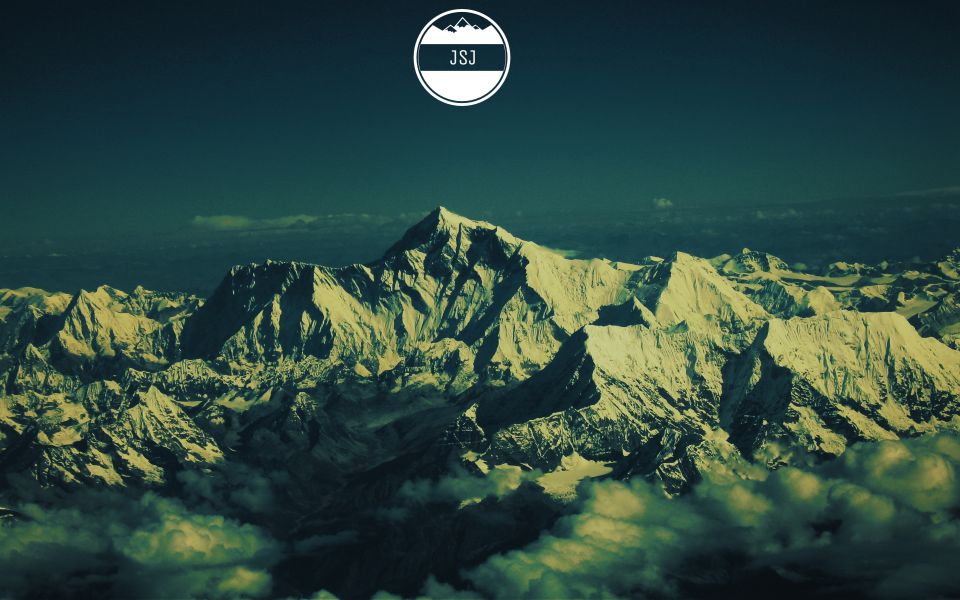
\includegraphics[width=\paperwidth]{imagenes/productos}};
\draw (current page.center) node [fill=ocre!30!white,fill opacity=0.6,text opacity=1,inner sep=1cm]{\Huge\centering\bfseries\sffamily\parbox[c][][t]{\paperwidth}{\centering JSJ Sport S.A.\\[15pt] % Book title
{\Large Tienda deportiva }\\[20pt] % Subtitle
{\huge Juan David Cubillos
\linebreak Juan Piedrahita}}}; % Author name
\end{tikzpicture}
\vfill
\endgroup

%%TABLA DE CONTENIDOS%%

\chapterimage{imagenes/tabla_contenido} % Table of contents heading image

\pagestyle{empty}

\tableofcontents

\cleardoublepage 

\pagestyle{fancy} 

\part{Proyecto}	
\chapter{Definición}


\section{Introducción}

En el mundo actual las pequeñas empresas se enfrentan día a día en el mercado, compiten por ganar prestigio y aumentar sus ganancias. Uno de los mayores problemas que se ven obligados a enfrentar estas pequeñas empresas es el de competir con grandes multinacionales, debido a que estas las dejan en una posición muy desfavorable a nivel de impacto y prestigio social debido a que cuentan con aliados que hacen que sus servicios sean más baratos e incluso mejores.
\newline
La mejor forma de lidiar con este problema es buscar siempre una innovación, una huella, un referente que haga que la empresa sea reconocida, es por esto que las empresas buscan abrir sus mercados y llegar al público de diferentes maneras. Muchas empresas aprovechan el auge de las redes sociales y el desarrollo del comercio web como una herramienta que le permite alcanzar nuevos mercados y de esta forma llegar a nuevos clientes potenciales.
\newline

%%\newpage

\section{Problema}

Debido a que muchas de las pequeñas empresas no cuentan con los medios necesarios en lo que se refiere a conocimientos y personal para poder empezar a comercializar sus productos por medio de una plataforma web se ven obligados a tercerizar estos servicios de forma que puedan llevarse a cabo sus objetivos.
\newline
Muchas de las empresas que se dedican a tercerizar servicios web no tienen en cuenta todas las necesidades de los clientes y solo se preocupan por realizar una plataforma web en la que se puedan mostrar y vender productos, se deja de lado la necesidad de los clientes de tener un control completo de los procesos de compra y venta e incluso de asesoría a sus clientes, es por eso que se hace necesario una empresa que se dedique a apoyar a este tipo de empresas ayudandolas a impulsarse en el mercado basándose en las nuevas tecnologías sin dejar de lado cada una de las necesidades de los clientes.

\newpage

\section{Objetivos}

\subsection{Objetivo General}

Brindar soluciones de tercerización de servicios para empresas que deseen expandir sus alcances en un entorno web con ayuda de las tecnologías emergentes.


\subsection{Objetivos Específicos}
\begin{itemize}
	\item Cumplir cada una de las necesidades de los clientes de forma que se plasme en un entorno web la forma en que prestan sus servicios.
	\item Usar tecnologías de vanguardia que permitan a nuestros clientes estar un paso adelante en el mercado actual. 
	\item Hacer del cliente una parte vital del equipo de trabajo durante el desarrollo del proyecto para que este tenga palabra y exprese sus necesidades.
	\item Brindar la máxima calidad posible a nuestros clientes por medio de productos altamente eficientes y con un excelente soporte.
\end{itemize}
%%\newpage

\section{Justificación}

Debido a la falta de preocupación de las diferentes empresas de tercerización de servicios web por las verdaderas necesidades del cliente cuando este intenta expandir su mercado por medio de un servicio o de una plataforma web que le permita llegar a diferentes públicos y expandir sus alcances, se hace necesaria una empresa que apoye al cliente y le brinde la asesoría requerida de forma que este se sienta incluido durante todo el proceso.
\newline

El desarrollo de una empresa que cumpla con estas características es de gran importancia para cada uno de los clientes que contratan sus servicios y quedan satisfechos con los productos que obtienen, su calidad y el proceso que se llevo a cabo para obtenerlos puesto que el se vio involucrado en este proceso y el producto se diseño conforme a sus necesidades y con su apoyo constante; pero no solo es importante por esto sino que también es importante para ayudar al desarrollo general de la economía de los diferentes sectores y de la región al contribuir a que se abran nuevas formas de mercado y los productos y servicios lleguen a públicos a los que antes no se tenia alcance, es decir que esta empresa también sera una importante herramienta para el desarrollo. 
%%\newpage

\section{Alcance}
Una vez sea definido el objeto de estudio, se planteara el diseño de una plataforma web de tipo e-commerce que le permita mostrar su producto y comercializarlo, la plataforma web contara inicialmente con las siguientes características:

\begin{enumerate}
	\item Información de contacto con la tienda.
	\item Muestra de los artículos y la cantidad disponible en bodega.
	\item Plataforma de pago en línea.
	\item Recibo de compra exitosa virtual.
\end{enumerate}

\subsection{Limitaciones}
El principal obstáculo de la realización de este proyecto es el tiempo de desarrollo para el mismo, por lo tanto para el primer prototipo se manejara un servicio de almacenamiento en base de datos local y no se creará un modulo que permita dar asesoría al cliente de la tienda en tiempo real.

\newpage

\section{Presuspuesto}

\begin{longtable}[c]{ccccc}
	\caption{Presupuesto}
	\label{tabla:presupuesto}\\
	\hline
	\multicolumn{5}{|l|}{\textbf{RECURSOS MATERIALES}}                                                                                                                                                                                                                                                                                                                                                                                                                                             \\ \hline
	\endfirsthead
	%
	\endhead
	%
	\multicolumn{1}{|c|}{\textbf{Recurso}}                                                                   & \multicolumn{1}{c|}{\textbf{Descripción}}                                                                                                                                                              & \multicolumn{1}{c|}{\textbf{Cantidad}} & \multicolumn{1}{c|}{\textbf{\begin{tabular}[c]{@{}c@{}}Valor \\ Unidad\end{tabular}}} & \multicolumn{1}{c|}{\textbf{Valor Total}} \\ \hline
	\multicolumn{1}{|c|}{\multirow{2}{*}{\begin{tabular}[c]{@{}c@{}}Computadores\\ Portátiles\end{tabular}}} & \multicolumn{1}{c|}{\begin{tabular}[c]{@{}c@{}}Procesador: Intel\\ Core i5\\ Memoria RAM:4gb\\ DD:500 GB\\ Pantalla 14''\end{tabular}}                                                                 & \multicolumn{1}{c|}{1}                 & \multicolumn{1}{c|}{\$1'500.000}                                                      & \multicolumn{1}{c|}{\$1'500.000}          \\ \cline{2-5} 
	\multicolumn{1}{|c|}{}                                                                                   & \multicolumn{1}{c|}{\begin{tabular}[c]{@{}c@{}}Procesador: Intel\\ Core i7\\ Memoria RAM: 6gb\\ DD: 1TB\\ Pantalla 14''\end{tabular}}                                                                  & \multicolumn{1}{c|}{1}                 & \multicolumn{1}{c|}{\$2'000.000}                                                      & \multicolumn{1}{c|}{\$2'000.000}          \\ \hline
	\multicolumn{1}{|c|}{\begin{tabular}[c]{@{}c@{}}Elementos de\\ Red\end{tabular}}                         & \multicolumn{1}{c|}{Internet}                                                                                                                                                                          & \multicolumn{1}{c|}{4 meses}           & \multicolumn{1}{c|}{\$60.000}                                                         & \multicolumn{1}{c|}{\$240.000}            \\ \hline
	\multicolumn{1}{|c|}{\multirow{2}{*}{licencias}}                                                         & \multicolumn{1}{c|}{Java}                                                                                                                                                                       & \multicolumn{1}{c|}{2}                 & \multicolumn{1}{c|}{\$0}                                                        & \multicolumn{1}{c|}{\$0}             \\ \cline{2-5} 
	\multicolumn{1}{|c|}{}                                                                                   & 
	\multicolumn{1}{c|}{MySQL}                                                                                                                                                                       & \multicolumn{1}{c|}{2}                 & \multicolumn{1}{c|}{\$0}                                                        & \multicolumn{1}{c|}{\$0}             \\ \cline{2-5} 
	\multicolumn{1}{|c|}{}                                                                                   &
	\multicolumn{1}{c|}{Eclipse}                                                                                                                                                                       & \multicolumn{1}{c|}{2}                 & \multicolumn{1}{c|}{\$0}                                                        & \multicolumn{1}{c|}{\$0}             \\ \cline{2-5} 
	\multicolumn{1}{|c|}{}                                                                                   &
	\multicolumn{1}{c|}{\begin{tabular}[c]{@{}c@{}} TeXstudio\end{tabular}}                                                                                                                 & \multicolumn{1}{c|}{2}                 & \multicolumn{1}{c|}{\$0}                                                              & \multicolumn{1}{c|}{\$0}                  \\                               
	 \hline
	\multicolumn{1}{|c|}{\begin{tabular}[c]{@{}c@{}}Centro de\\ Desarrollo y \\ oficina\end{tabular}}        & \multicolumn{1}{c|}{\begin{tabular}[c]{@{}c@{}}Espacio fisico \\ donde se llevará a \\ cabo todo el\\ desarrollo del\\ proyecto\end{tabular}}                                                          & \multicolumn{1}{c|}{4 meses}           & \multicolumn{1}{c|}{\$1'000.000}                                                      & \multicolumn{1}{c|}{\$4'000.000}          \\ \hline
	\multicolumn{1}{|c|}{\multirow{4}{*}{Equipo Oficina}}                                                    & \multicolumn{1}{c|}{Escritorios}                                                                                                                                                                       & \multicolumn{1}{c|}{4}                 & \multicolumn{1}{c|}{\$300.000}                                                        & \multicolumn{1}{c|}{\$1'200.000}          \\ \cline{2-5} 
	\multicolumn{1}{|c|}{}                                                                                   & \multicolumn{1}{c|}{Sillas}                                                                                                                                                                            & \multicolumn{1}{c|}{4}                 & \multicolumn{1}{c|}{\$50.000}                                                         & \multicolumn{1}{c|}{\$200.000}            \\ \cline{2-5} 
	\multicolumn{1}{|c|}{}                                                                                   & \multicolumn{1}{c|}{\begin{tabular}[c]{@{}c@{}}Scanner e \\ Impresora\end{tabular}}                                                                                                                    & \multicolumn{1}{c|}{1}                 & \multicolumn{1}{c|}{\$150.000}                                                        & \multicolumn{1}{c|}{\$150.000}            \\ \cline{2-5} 
	\multicolumn{1}{|c|}{}                                                                                   & \multicolumn{1}{c|}{\begin{tabular}[c]{@{}c@{}}Papeleria y utiles\\ de Oficina\end{tabular}}                                                                                                           & \multicolumn{1}{c|}{1}                 & \multicolumn{1}{c|}{\$400.000}                                                        & \multicolumn{1}{c|}{\$400.000}            \\ \hline
	\multicolumn{5}{|l|}{\textbf{Recursos Humanos}}                                                                                                                                                                                                                                                                                                                                                                                                                                                \\ \hline
	\multicolumn{1}{|c|}{Desarrolladores}                                                                      & \multicolumn{1}{c|}{\begin{tabular}[c]{@{}c@{}}Desarrollo del \\ proyecto: \\ análisis de\\ requerimientos\\  consecuentes con \\ los objetivos, \\ restricciones y\\ alcances planteados \\ y codificación y \\ pruebas\end{tabular}}      & \multicolumn{1}{c|}{2}                 & \multicolumn{1}{c|}{\$12'000.000}                                                      & \multicolumn{1}{c|}{\$24'000.000}         \\ \hline

	\multicolumn{1}{|c|}{\begin{tabular}[c]{@{}c@{}}Total del \\ Proyecto\end{tabular}}                      & \multicolumn{4}{r|}{\$33'690.000}                                                                                                                                                                                                                                                                                                                                                                               \\ \hline
                                                                                                                                                                                                                                                                                               
\end{longtable}

\chapter{Metodología}
\section{Introducción}

La finalidad de definir desde el principio una metodoligía y hacer uso de esta durante todo el desarrollo es la de hacer más eficaz el proceso de desarrollo del producto y lograr una alta calidad de forma que sea costeable tanto para el equipo de trabajo como para el cliente mismo, la metodología también define las reglas de trabajo para el grupo que llevara a cabo el desarrollo, las actividades y los procesos que este grupo debe realizar y la forma en que debe realizarlos.
\newline
Para este caso en especifico se busca una metodología de trabajo que principalmente incluya al cliente como una de las partes fundamentales del desarrollo y permita al equipo estar en constante comunicación con este, la metodología debe permitir atender requerimientos emergentes y ademas la metodología escogida debe permitir mostrar al cliente los avances desarrollados en un período de tiempo de forma que este pueda hacer comentarios y exprese su satisfacción o informe en caso de que no este conforme con algo.
\newpage

\section{Prototipo}
Para el desarrollo de la plataforma web, se utilizara la metodología "Prototipo para desarrollo del software", la cual consta de una fase de requerimientos y de diseño con la creación de un subproducto, es esto lo que llamamos prototipo ya que es una fase temprana del mismo para ver su comportamiento, posteriormente se realiza una fase de implementación, una pruebas y una final de mantenimiento.
\newline
Además de esto se escoge esta metodología puesto que esta permite al cliente ser parte del proceso de desarrollo viendo el avance que este lleva y haciendo las observaciones pertinentes desde su punto de vista, de forma que se crea un dialogo entre el equipo de desarrollo y el cliente que permite establecer mejor las funcionalidades que se espera tenga el producto final y los requisitos que debe cumplir. Esto mejora la calidad del producto asegurando que este cumpla con las expectativas del cliente.
\begin{figure}[th!]
	\centering
	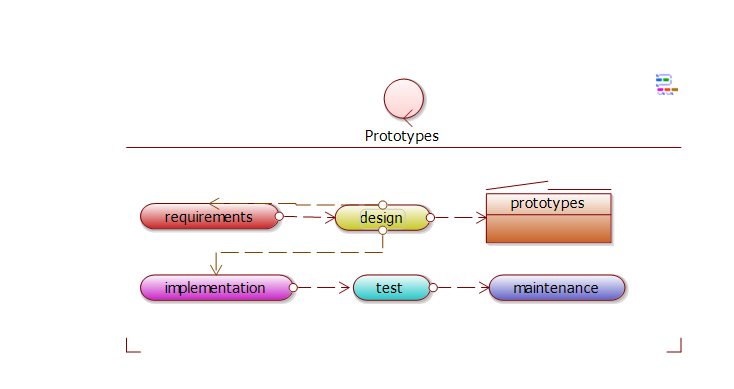
\includegraphics[width=0.9\linewidth]{imagenes/Proceso1}
	\caption{Proceso de desarrollo de software: Prototipo}
\end{figure}

\newpage

\section{Cronograma}

Teniendo claro la metodología a utilizar, se procede a organizar el tiempo requerido para realizar el desarrollo del proyecto, teniendo en cuenta la cantidad de semanas destinadas para el desarrollo completo del prototipo y la documentación pertinente.

\begin{figure}[th!]
	\centering
	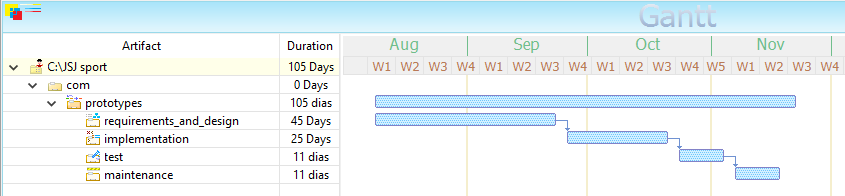
\includegraphics[width=0.9\linewidth]{imagenes/cronograma}
	\caption{Proceso de desarrollo de software: Prototipo}
\end{figure}


\newpage

\part{Arquitectura y Diseño}
\chapter{Empresa}

\section{Introducción}

\newpage

\section{Nombre -RS-}


\section{Misión}


\section{Visión}

\newpage

\section{Objetivos}

estos objetivos deben ser operacionales

\newpage



\chapter{ADM}


\section{Introdución}

TOGAF ADM (Architecture Development Method) forma el centro de TOGAF. ADM es el resultado de contribuciones continuas de un gran número de arquitecturas, también describe un método para desarrollar y administrar el ciclo de vida de una arquitectura empresarial, ademas se apoya en muchos de los elementos de TOGAF y recursos de otras arquitecturas que están disponibles con el fin de conocer el negocio y las TI que de una organización.
\newline
El framework de TOGAF se complementa de Archimate puesto que este proporciona un conjunto independiente de conceptos, incluyendo una representación gráfica, que ayuda a crear un modelo coherente e integrado  "por debajo de la linea de flotación" que se puede representar en forma de vistas TOGAF, es por eso que en el desarrollo de este capitulo se explicara el uso de ADM, sus puntos claves y las integración que se da con Archimate desde las diferentes capas que este tiene.

\newpage

\section{Arquitectura base de una empresa}

ADM es útil para describir la Arquitectura Base de una empresa. Los requisitos empresariales que se tienen se pueden utilizar para identificar las definiciones y selecciones necesarias en la base de la arquitectura. Estos requisitos pueden ser un conjunto de modelos comunes reutilizables, políticas y definiciones de gobernabilidad, o incluso pueden ser algo mas especifico como selecciones tecnológicas sobresaliente. Al realizar la descripción de la Arquitectura Base se sigue principios similares a los de una arquitectura empresarial, con la diferencia de que los requisitos para toda una empresa se limitan a las preocupaciones generales y, por tanto, es menos completo que para una parte de la empresa específica.

\subsection{Puntos clavede ADM}

\begin{itemize}
	\item ADM es iterativo, a lo largo de todo el proceso, entre las fases, y dentro de las fases . Para cada interacción de la ADM, una nueva decisión debe ser tomada en base a:
	\begin{itemize}
		\item La amplitud de la cobertura de la empresa que se define.
		\item El nivel de detalle que se define.
		\item La extensión del período de tiempo destinado, incluyendo el número y la extensión de los períodos de tiempo intermedios.
		\item Los activos de arquitectura para ser aprovechados, incluyendo:
		\begin{itemize}
			\item Activos creados en versiones anteriores del ciclo de ADM dentro de la empresa.
			\item Activos disponibles en otras partes de la industria (otros marcos, modelos de sistemas, modelos verticales de la industria, etc.).
		\end{itemize}
	\end{itemize}
	\item Las decisiones tomadas en cada fase se deben basar en una evaluación práctica de los recursos y la disponibilidad de competencias, y en el valor que realmente se puede esperar recibir de la empresa en el ámbito elegido del trabajo de la arquitectura.
	\item Como un método genérico, ADM está destinado a ser utilizado por empresas en una amplia variedad de diferentes zonas geográficas y aplicado en diferentes tipos sectores / industria vertical. Como tal, puede ser, pero no necesariamente tiene que ser, adaptado a las necesidades específicas.
\end{itemize}

\newpage
\subsection{Modelo de proceso ADM}

Es importante recalcar que a lo largo del ciclo ADM, es necesario que se evaluen los resultados contra las expectativas originales, esto tanto para el ciclo ADM completo como para cada fase particular del proceso.

\begin{figure}[h]
	\centering
	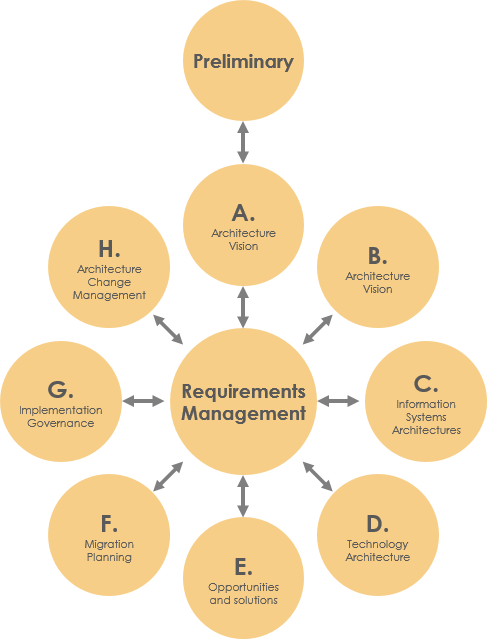
\includegraphics[width=0.7\linewidth]{arquitectura/imagenes/modeloADM}
	\caption{Estructura base del Modelo de Proceso de ADM }
	\label{fig:modeloadm}
\end{figure}
\newpage


\section{ArchiMate}

ArchiMate es un lenguaje de modelado de arquitectura empresarial abierto e independiente que soporta la descripción, análisis y visualización de las relaciones entre los diferentes dominios de negocios de una forma no ambigua, es deccir, la especificación de ArchiMate define un lenguaje común para describir la construcción y operación de procesos de negocios, estructuras organizacionales, flujos de información, sistemas de TI e infraestructura técnica. Esta visión ayuda a las partes interesadas a diseñar, evaluar y comunicar las consecuencias de las decisiones y cambios dentro y entre los dominios de negocio.  
\newline
Con su versión mas reciente ArchiMate 3.0 de 2016, se puede modelar la empresa a un nivel estratégico, como capacidad, recursos y resultados. También se incluye el apoyo para modelar el mundo físico de materiales y equipos.
\newline
ArchiMate se divide en capas como se puede observar en la siguiente figura:
\newline

\begin{figure} [h]
	\centering
	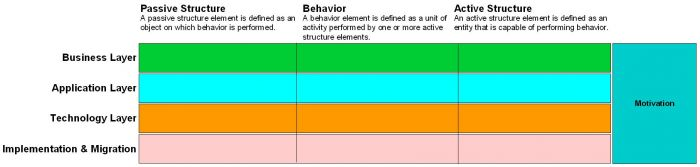
\includegraphics[width=0.7\linewidth]{arquitectura/imagenes/Archimate}
	\caption{Estructura por capas de ArchiMate}
	\label{fig:archimate}
\end{figure}

A continuación se van a mostrar los conceptos de las diferentes capas que se utilizan para el modelamiento en ArchiMate, dentro de las que se encuentran Capa de Negocio, Capa de Aplicación, Capa de Tecnologías, Capa de Motivación y Capa de Migración, además de esto también se mostrara la tabla de Relaciones.

\newpage

\subsection{Capa de negocio}

Se refiere a los procesos de negocio, servicios, funciones y eventos ce cada una de las unidades de negocio. Esta capa ofrece productos y servicios a clientes externos, que se realizan en la organización mediante procesos de negocio realizados por actores y roles empresariales.

\begin{table}[H]
	\centering\textbf{TABLA DE CONCEPTOS CAPA DE NEGOCIO}

	\centering
	\begin{tabular}{| m{4cm} | m{4cm} | m{4cm} | }
		\hline
		\centering\vspace{1.52mm}CONCEPTO & \centering\vspace{1.52mm}DESCRIPCION & \vspace{1.52mm}NOTACION \\
		\hline
		\centering\vspace{1.52mm}Actor de Negocio & \vspace{1.52mm} Una entidad de organización que es capaz de comportamiento artístico. & \vspace{1.52mm}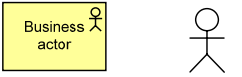
\includegraphics[width=40mm]{arquitectura/imagenes/11} \\
		\hline
		\centering\vspace{1.52mm}Rol de Negocio & \vspace{1.52mm} La responsabilidad de realizar el comportamiento específico, al cual un actor puede ser asignado.  & \vspace{1.52mm}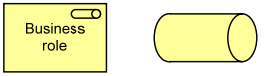
\includegraphics[width=40mm]{arquitectura/imagenes/12} \\
		\hline
		\centering\vspace{1.52mm}Colaboración de Negocio & \vspace{1.52mm}Un conjunto de dos o más papeles de negocio que trabajan juntos para realizar el comportamiento colectivo.   & \vspace{1.52mm}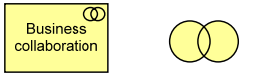
\includegraphics[width=40mm]{arquitectura/imagenes/13} \\
		\hline
		\centering\vspace{1.52mm}Interfaz de Negocio & \vspace{1.52mm}Un punto de acceso donde un servicio de gestión es hecho disponible al entorno.   & \vspace{1.52mm}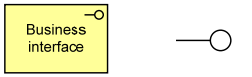
\includegraphics[width=40mm]{arquitectura/imagenes/14} \\
		\hline
		\centering\vspace{1.52mm}Ubicación & \vspace{1.52mm}Un punto conceptual o ampliado en espacio.& \vspace{1.52mm}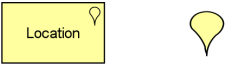
\includegraphics[width=40mm]{arquitectura/imagenes/15} \\
		\hline
		\centering\vspace{1.52mm}Objeto de Negocio & \vspace{1.52mm}Un elemento pasivo que tiene la importancia de una perspectiva de negocio. & \vspace{1.52mm}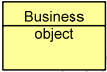
\includegraphics[width=20mm]{arquitectura/imagenes/16} \\
		\hline
		\centering\vspace{1.52mm}Proceso de Negocio & \vspace{1.52mm}Un elemento de comportamiento de grupos basado en un ordenamiento de actividades. Es querido para producir un juego definido de productos o servicios de gestión. & \vspace{1.52mm}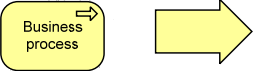
\includegraphics[width=40mm]{arquitectura/imagenes/17} \\
		\hline
		\centering\vspace{1.52mm}Función de Negocio & \vspace{1.52mm}Un elemento de comportamiento de grupos basado en un juego escogido de criterios (recursos típicamente requeridos de negocio y/o competencias).  & \vspace{1.52mm}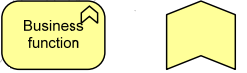
\includegraphics[width=40mm]{arquitectura/imagenes/18} \\
		\hline
	\end{tabular}
\end{table}

\begin{table}[H]
	\centering
	\begin{tabular}{| m{4cm} | m{4cm} | m{4cm} | }
		\hline
		\centering\vspace{1.52mm}CONCEPTO & \centering\vspace{1.52mm}DESCRIPCION &\vspace{1.52mm}NOTACION \\
		\hline
		\centering\vspace{1.52mm}Interacción de Negocio & \vspace{1.52mm}Un elemento de comportamiento que describe el comportamiento de una colaboración de negocio.   & \vspace{1.52mm}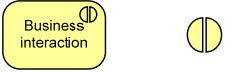
\includegraphics[width=40mm]{arquitectura/imagenes/19} \\
		\hline
		\centering\vspace{1.52mm}Evento de Negocio & \vspace{1.52mm}Algo qué pasa (internamente o por fuera) e influye en el comportamiento. & \vspace{1.52mm}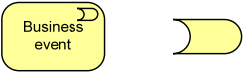
\includegraphics[width=40mm]{arquitectura/imagenes/110} \\
		\hline
		\centering\vspace{1.52mm}Servicio de Negocio & \vspace{1.52mm}Un servicio que realiza una necesidad de negocio de un cliente (interno o externo a la organización). & \vspace{1.52mm}
\includegraphics[width=40mm]{arquitectura/imagenes/111} \\
		\hline
		\centering\vspace{1.52mm}Representación & \vspace{1.52mm}Una forma perceptible de la información llevada por un objeto de negocio. & \vspace{1.52mm}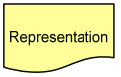
\includegraphics[width=20mm]{arquitectura/imagenes/112} \\
		\hline
		\centering\vspace{1.52mm}Significado & \vspace{1.52mm}El conocimiento o la experiencia se presentan en un objeto de negocio o su representación, considerando un contexto particular. & \vspace{1.52mm}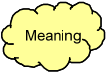
\includegraphics[width=20mm]{arquitectura/imagenes/113} \\
		\hline
		\centering\vspace{1.52mm}Valor & \vspace{1.52mm}El valor de pariente, utilidad, o importancia de un servicio de gestión o producto. & \vspace{1.52mm}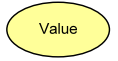
\includegraphics[width=25mm]{arquitectura/imagenes/114} \\
		\hline
		\centering\vspace{1.52mm}Producto & \vspace{1.52mm}Una colección coherente de servicios, acompañados por un contraer/poner de acuerdos, que ofrecen en total (a interno o externo) a clientes. & \vspace{1.52mm}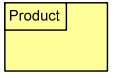
\includegraphics[width=20mm]{arquitectura/imagenes/115} \\
		\hline
		\centering\vspace{1.52mm}Contrato & \vspace{1.52mm}Una especificación formal o informal de acuerdo que especifica los derechos y obligaciones asociadas con un producto. & \vspace{1.52mm}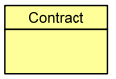
\includegraphics[width=20mm]{arquitectura/imagenes/116} \\
		\hline
	\end{tabular}
	\caption{Tabla de Conceptos de la Capa de Negocio}
	\label{fig:negocio}
\end{table}

\subsection{Capa de Aplicación}

Se trata de aplicaciones de software que "soportan los componentes de la empresa con servicios de aplicación".

\begin{table}[H]
	\centering\textbf{TABLA CONCEPTOS CAPA DE APLICACIÓN}
	\centering
	\begin{tabular}{| m{4cm} | m{4cm} | m{4cm} | }
		\hline
		\centering\vspace{1.52mm}CONCEPTO & \centering\vspace{1.52mm}DESCRIPCION &\vspace{1.52mm}NOTACION \\
		\hline
		\centering\vspace{1.52mm}Componente de Aplicación & \vspace{1.52mm}Una parte modular, desplegable, y reemplazable de un sistema de software que encapsula su comportamiento y datos y expone estos por un juego de interfaces.& \vspace{1.52mm}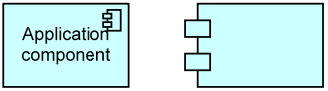
\includegraphics[width=40mm]{arquitectura/imagenes/21} \\
		\hline
		\centering\vspace{1.52mm}Colaboración de Aplicación & \vspace{1.52mm}Un conjunto de dos o más componentes de aplicación que trabajan juntos para realizar el comportamiento colectivo.& \vspace{1.52mm}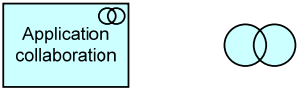
\includegraphics[width=40mm]{arquitectura/imagenes/22} \\
		\hline
		\centering\vspace{1.52mm}Interfaz de Aplicación & \vspace{1.52mm}Un punto de acceso donde un servicio de aplicación es hecho disponible a un usuario u otro componente de aplicación.& \vspace{1.52mm}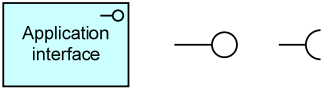
\includegraphics[width=40mm]{arquitectura/imagenes/23} \\
		\hline
		\centering\vspace{1.52mm}Objeto de Datos & \vspace{1.52mm}Un elemento pasivo conveniente para tratamiento automatizado.& \vspace{1.52mm}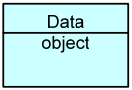
\includegraphics[width=20mm]{arquitectura/imagenes/24} \\
		\hline
		\centering\vspace{1.52mm}Función de Aplicación & \vspace{1.52mm}Un elemento de comportamiento que los grupos automatizaron el comportamiento que puede ser realizado por un componente de aplicación.& \vspace{1.52mm}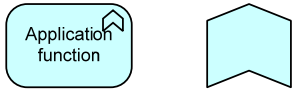
\includegraphics[width=40mm]{arquitectura/imagenes/25} \\
		\hline
		\centering\vspace{1.52mm}Interacción de Aplicación & \vspace{1.52mm}Un elemento de comportamiento que describe el comportamiento de una colaboración de aplicación.& \vspace{1.52mm}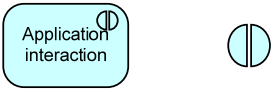
\includegraphics[width=40mm]{arquitectura/imagenes/26} \\
		\hline
		\centering\vspace{1.52mm}Servicio de Aplicación & \vspace{1.52mm}Un servicio que expone el comportamiento automatizado.& \vspace{1.52mm}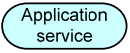
\includegraphics[width=20mm]{arquitectura/imagenes/27} \\
		\hline
	\end{tabular}
	\caption{Tabla de Conceptos de la Capa de Aplicación}
	\label{fig:aplicacion}
\end{table}

\subsection{Capa de Tecnologías}

Esta capa "Trata con la infraestructura de hardware y comunicación para soportar la Capa de Aplicación, esta capa ofrece servicios de infraestructura necesarios para ejecutar aplicaciones, realizadas por computadora y hardware de comunicación y software de sistema ".


\begin{table}[H]
	\centering\textbf{TABLA CONCEPTOS CAPA DE TECNOLOGIAS}
	\centering
	\begin{tabular}{| m{4cm} | m{4cm} | m{4cm} | }
		\hline
		\centering\vspace{1.52mm}CONCEPTO & \centering\vspace{1.52mm}DESCRIPCION &\vspace{1.52mm}NOTACION \\
		\hline
		\centering\vspace{1.52mm}Nodo & \vspace{1.52mm}Un recurso computacional con lo cual los artefactos pueden ser almacenados o desplegados para la ejecución.& \vspace{1.52mm}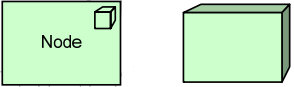
\includegraphics[width=40mm]{arquitectura/imagenes/31} \\
		\hline
		\centering\vspace{1.52mm}Dispositivo & \vspace{1.52mm}Un recurso de hardware con lo cual los artefactos pueden ser almacenados o desplegados para la ejecución.& \vspace{1.52mm}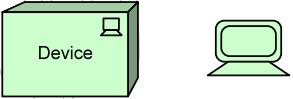
\includegraphics[width=40mm]{arquitectura/imagenes/32} \\
		\hline
		\centering\vspace{1.52mm}Red & \vspace{1.52mm}Un medio de comunicación entre dos o más dispositivos.& \vspace{1.52mm}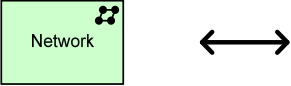
\includegraphics[width=40mm]{arquitectura/imagenes/33} \\
		\hline
		\centering\vspace{1.52mm}Camino de Comunicación & \vspace{1.52mm}Un eslabón entre dos o más nodos, por los cuales estos nodos pueden cambiar datos.& \vspace{1.52mm}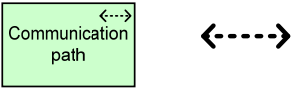
\includegraphics[width=40mm]{arquitectura/imagenes/34} \\
		\hline
		\centering\vspace{1.52mm}Interface de Infraestructura & \vspace{1.52mm}Un punto de acceso donde los servicios de infraestructura ofrecidos por un nodo pueden ser tenidos acceso por otros nodos y componentes de aplicación. & \vspace{1.52mm}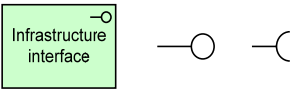
\includegraphics[width=40mm]{arquitectura/imagenes/35} \\
		\hline
		\centering\vspace{1.52mm}Sistema de Software & \vspace{1.52mm}Un entorno de software para los tipos específicos de componentes y objetos que son desplegados sobre ello en forma de artefactos.& \vspace{1.52mm}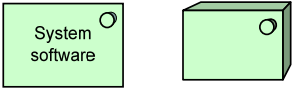
\includegraphics[width=40mm]{arquitectura/imagenes/36} \\
		\hline
		\centering\vspace{1.52mm}Función de Infraestructura & \vspace{1.52mm}Un elemento de comportamiento de grupos el comportamiento infraestructural puede ser realizado por un nodo.& \vspace{1.52mm}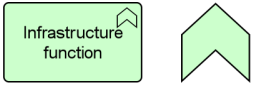
\includegraphics[width=40mm]{arquitectura/imagenes/37} \\
		\hline
		\centering\vspace{1.52mm}Servicios de Infraestructura & \vspace{1.52mm}Una unidad por fuera visible de funcionalidad, a condición de que por uno o varios nodos, expuestos por interfaces bien definidos, y significativo al entorno.& \vspace{1.52mm}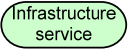
\includegraphics[width=20mm]{arquitectura/imagenes/38} \\
		\hline
	\end{tabular}
\end{table}

\begin{table}[H]
	\centering
	\begin{tabular}{| m{4cm} | m{4cm} | m{4cm} | }
		\hline
		\centering\vspace{1.52mm}CONCEPTO & \centering\vspace{1.52mm}DESCRIPCION &\vspace{1.52mm}NOTACION \\
		\hline
		\centering\vspace{1.52mm}Artefacto & \vspace{1.52mm}Un pedazo físico de los datos que es usado o producido en un proceso de desarrollo de software, o por el despliegue y la operación de un sistema.& \vspace{1.52mm}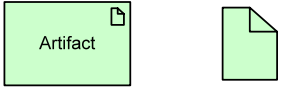
\includegraphics[width=40mm]{arquitectura/imagenes/39} \\
		\hline
	\end{tabular}
	\caption{Tabla de Conceptos de la Capa de Tecnologías}
	\label{fig:tecnologias}
\end{table}

\subsection{Capa de Motivación}

Los conceptos de motivación se utilizan para modelar las motivaciones, o razones, que subyacen en el diseño o cambio de alguna arquitectura empresarial. Estas motivaciones afectan, orientan y limitan el diseño.


\begin{table}[H]
	\centering\textbf{TABLA DE CONCEPTOS CAPA DE MOTIVACIÓN}
	\centering
	\begin{tabular}{| m{4cm} | m{4cm} | m{4cm} | }
		\hline
		\centering\vspace{1.52mm}CONCEPTO & \centering\vspace{1.52mm}DESCRIPCION &\vspace{1.52mm}NOTACION \\
		\hline
		\centering\vspace{1.52mm}Tenedor de Apuestas& \vspace{1.52mm}El papel de un individuo, el equipo, o la organización (o clasifica de eso) que representa sus intereses a, o concierne en relación con, el resultado de la arquitectura.& \vspace{1.52mm}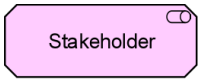
\includegraphics[width=30mm]{arquitectura/imagenes/51} \\
		\hline
		\centering\vspace{1.52mm}Conductor& \vspace{1.52mm}Algo qué crea, motiva, y abastece de combustible el cambio de una organización.& \vspace{1.52mm}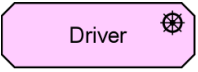
\includegraphics[width=30mm]{arquitectura/imagenes/52} \\
		\hline
		\centering\vspace{1.52mm}Evaluación& \vspace{1.52mm}El resultado de algún análisis de algún conductor.& \vspace{1.52mm}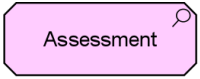
\includegraphics[width=30mm]{arquitectura/imagenes/53} \\
		\hline
		\centering\vspace{1.52mm}Objetivo& \vspace{1.52mm}Un estado de final que un tenedor de apuestas tiene la intención de alcanzar.& \vspace{1.52mm}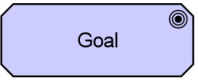
\includegraphics[width=30mm]{arquitectura/imagenes/54} \\
		\hline
		\centering\vspace{1.52mm}Requerimientos& \vspace{1.52mm}Una declaración de necesidad que debe ser realizada por un sistema.& \vspace{1.52mm}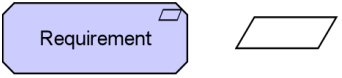
\includegraphics[width=40mm]{arquitectura/imagenes/55} \\
		\hline
		\centering\vspace{1.52mm}Coacción& \vspace{1.52mm}Una restricción en el camino en la cual un sistema es realizado.& \vspace{1.52mm}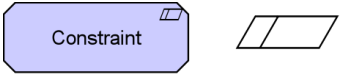
\includegraphics[width=40mm]{arquitectura/imagenes/56} \\
		\hline
		\centering\vspace{1.52mm}Principio& \vspace{1.52mm}Una propiedad normativa de todos los sistemas en un contexto dado, o el camino en cual ellos son realizados.& \vspace{1.52mm}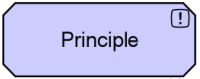
\includegraphics[width=30mm]{arquitectura/imagenes/57} \\
		\hline
	\end{tabular}
	\caption{Tabla de Conceptos de Capa Motivación}
	\label{fig:motivacion}
\end{table}

\subsection{Capa de Implementación y  Migración}

 Es similar a un proceso de negocio, en el sentido de que consiste en un conjunto de tareas relacionadas causalmente, dirigidas a producir un resultado bien definido.

\begin{table}[H]
	\centering\textbf{TABLA DE CONCEPTOS CAPA DE IMPLEMENTACIÓN Y MIGRACIÓN}
	\centering
	\begin{tabular}{| m{4cm} | m{4cm} | m{4cm} | }
		\hline
		\centering\vspace{1.52mm}CONCEPTO & \centering\vspace{1.52mm}DESCRIPCION &\vspace{1.52mm}NOTACION \\
		\hline
		\centering\vspace{1.52mm}Paquete de Trabajo& \vspace{1.52mm}Una serie de acciones diseñadas para lograr un objetivo único dentro de un tiempo especificado.& \vspace{1.52mm}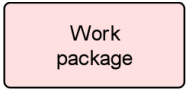
\includegraphics[width=25mm]{arquitectura/imagenes/61} \\
		\hline
		\centering\vspace{1.52mm}Entregable& \vspace{1.52mm}Un resultado definido con precisión de un paquete de trabajo.& \vspace{1.52mm}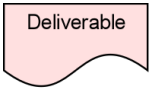
\includegraphics[width=20mm]{arquitectura/imagenes/62} \\
		\hline
		\centering\vspace{1.52mm}Meseta& \vspace{1.52mm}Un estado relativamente estable de la arquitectura que existe durante un período limitado de tiempo.& \vspace{1.52mm}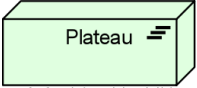
\includegraphics[width=25mm]{arquitectura/imagenes/63} \\
		\hline
		\centering\vspace{1.52mm}Objetivo& \vspace{1.52mm}Un resultado de un análisis de hueco entre dos mesetas.& \vspace{1.52mm}\includegraphics[width=25mm]{arquitectura/imagenes/64} \\
		\hline
	\end{tabular}
	\caption{Tabla de Conceptos de Capa Migración}
	\label{fig:migracion}
\end{table}

\subsection{Tabla de relaciones}

\begin{table}[H]
	\centering\textbf{TABLA DE RELACIONES}
	\centering
	\begin{tabular}{| m{4cm} | m{4cm} | m{4cm} | }
		\hline
		\centering\vspace{1.52mm}CONCEPTO & \centering\vspace{1.52mm}DESCRIPCION &\vspace{1.52mm}NOTACION \\
		\hline
		&\centering\vspace{1.52mm}RELACIONES ESTRUCTURALES & \\
		\hline
		\centering\vspace{1.52mm}Asociación & \vspace{1.52mm}La asociación modela una relación entre los objetos que no es cubierta por el otro, la relación más específica.& \vspace{1.52mm}\includegraphics[width=40mm]{arquitectura/imagenes/41} \\
		\hline
		\centering\vspace{1.52mm}Acceso & \vspace{1.52mm}La relación de acceso modela el acceso de conceptos conductuales a objetos de datos o el negocio.& \vspace{1.52mm}\includegraphics[width=40mm]{arquitectura/imagenes/42} \\
		\hline
		\centering\vspace{1.52mm}Usado Por & \vspace{1.52mm}El usado por la relación modela el empleo de servicios por procesos, funciones, o interacciones y el acceso a interfaces por papeles, componentes, o colaboraciones.& \vspace{1.52mm}\includegraphics[width=30mm]{arquitectura/imagenes/43} \\
		\hline
	\end{tabular}
\end{table}

\begin{table}[H]
	\centering
	\begin{tabular}{| m{4cm} | m{4cm} | m{4cm} | }
		\hline
		\centering\vspace{1.52mm}CONCEPTO & \centering\vspace{1.52mm}DESCRIPCION &\vspace{1.52mm}NOTACION \\
		\hline
		\centering\vspace{1.52mm}Realización & \vspace{1.52mm}La relación de realización une una entidad lógica con más entidad concreta que lo realiza.& \vspace{1.52mm}\includegraphics[width=30mm]{arquitectura/imagenes/44} \\
		\hline
		\centering\vspace{1.52mm}Asignación & \vspace{1.52mm}La relación de asignación une las unidades de comportamiento con elementos activos (p.ej., papeles, componentes) que los realiza, o papeles con los actores que los realizan.& \vspace{1.52mm}\includegraphics[width=30mm]{arquitectura/imagenes/45} \\
		\hline
		\centering\vspace{1.52mm}Agregación & \vspace{1.52mm}La relación de agregación indica que un objeto agrupa un número de otros objetos.& \vspace{1.52mm}\includegraphics[width=30mm]{arquitectura/imagenes/46} \\
		\hline
		\centering\vspace{1.52mm}Composición & \vspace{1.52mm}La relación de composición indica que un objeto es compuesto de uno o varios otros objetos.& \vspace{1.52mm}\includegraphics[width=30mm]{arquitectura/imagenes/47} \\
		\hline
		&\centering\vspace{1.52mm}RELACIONES DINAMICAS & \\
		\hline
		\centering\vspace{1.52mm}Flujo & \vspace{1.52mm}La relación de flujo describe la transferencia de, por ejemplo, la información o el valor entre procesos, función, interacciones, y acontecimientos.& \vspace{1.52mm}\includegraphics[width=30mm]{arquitectura/imagenes/48} \\
		\hline
		\centering\vspace{1.52mm}Provocación& \vspace{1.52mm}La relación de provocación describe las relaciones temporales o causales entre procesos, funciones, interacciones, y acontecimientos.& \vspace{1.52mm}\includegraphics[width=30mm]{arquitectura/imagenes/49} \\
		\hline
		&\centering\vspace{1.52mm}OTRAS RELACIONES & \\
		\hline
		\centering\vspace{1.52mm}Agrupación& \vspace{1.52mm}La relación que de agrupación indica que los objetos, del mismo tipo o tipos diferentes, pertenecen juntos basado en alguna característica común.& \vspace{1.52mm}\includegraphics[width=20mm]{arquitectura/imagenes/410} \\
		\hline
		\centering\vspace{1.52mm}Unión& \vspace{1.52mm}Una unión es usada para unir las relaciones del mismo tipo.& \vspace{1.52mm}\includegraphics[width=20mm]{arquitectura/imagenes/411} \\
		\hline
		\centering\vspace{1.52mm}Especialización& \vspace{1.52mm}La relación de especialización indica que un objeto es una especialización de otro objeto.& \vspace{1.52mm}\includegraphics[width=20mm]{arquitectura/imagenes/412} \\
		\hline
	\end{tabular}
	\caption{Tabla de Relaciones}
	\label{fig:relaciones}
\end{table}


\section{Intergación AMD y ArchiMate}

\begin{figure}[h]
	\centering
	\includegraphics[width=0.7\linewidth]{arquitectura/imagenes/AMD_ArchiMate}
	\caption{Relación entre AMD y ArchiMate}
	\label{fig:amdarchimate}
\end{figure}


Como se logra ver en la imagen la estructura del lenguaje central de ArchiMate se relaciona estrechamente con las arquitecturas principales de TOGAF ADM. Los elementos de estrategia, motivación, implementación y migración se correlacionan aproximadamente con el resto de ADM (aunque estos elementos también pueden usarse en las Fases B, C y D). Esta correspondencia indica una asignación bastante fácil entre las vistas TOGAF y los puntos de vista de ArchiMate.
\newline
Aunque algunos de los puntos de vista que se definen en el estándar TOGAF no se pueden asignar fácilmente a los puntos de vista de ArchiMate, el lenguaje ArchiMate y sus técnicas de análisis soportan los conceptos abordados en estos puntos de vista. Aunque no existe una correspondencia entre uno y otro, todavía hay una buena cantidad de correspondencia entre los puntos de vista de ArchiMate y los puntos de vista de TOGAF.
\newline
Los estándares de TOGAF y ArchiMate pueden usarse de forma fácil debido a que:

\begin{itemize}
	\item Los dos estándares se complementan entre sí con respecto a la definición de un proceso de desarrollo de arquitectura y la definición de un lenguaje de modelado de Arquitectura Empresarial.
	\item Las dos normas se superponen en su uso de los puntos de vista, y el concepto de un repositorio común subyacente de artefactos y modelos arquitectónicos; Es decir, tienen una base común firme.
	\item El uso combinado de las dos normas puede apoyar una mejor comunicación con las partes interesadas.
\end{itemize}


\newpage



\chapter{Negocio}

\section{Introducción}

Esta capa se refiere a los procesos de negocio, servicios, funciones y eventos ce cada una de las unidades de negocio. Esta capa ofrece productos y servicios a clientes externos, que se realizan en la organización mediante procesos de negocio realizados por actores y roles empresariales.

\begin{figure}[th!]
	\centering
	\includegraphics[width=0.6\linewidth]{arquitectura/imagenes/negocio}
	\caption{Metamodelo de la capa de negocio }
	\label{fig:negocio}
\end{figure}

La capa de negocio contiene la lógica principal de procesamiento de datos dentro de nuestra aplicación Web. Se comunica con la capa de presentación para obtener las entradas del usuario y presentar la información resultante, así como la capa de acceso a datos o directamente con servicios para realizar sus operaciones.

\newpage

\section{Punto de Vista de Organización}

\subsection{Modelo}
\begin{figure}[th!]
	\centering
	\includegraphics[width=0.5\linewidth]{arquitectura/imagenes/modeloOrganizacion}
	\caption{Metamodelo de Punto de Vista de Organización  \cite{pun1}}
	\label{fig:metamodelo de punto de vista de organizacion}
\end{figure}
El punto de vista de la organización se centra en la organización (interna) de una empresa, un departamento, una red de empresas o de otra entidad organizativa. Es posible presentar modelos en este punto de vista como diagramas de bloques anidados, pero también de una manera más tradicional, como los organigramas. El punto de vista de la Organización es muy útil  en la identificación de competencias, autoridad y responsabilidades en una organización.


\subsection{Caso de estudio}


\begin{figure}[!th]
	\centering
	\includegraphics[width=0.5\linewidth]{arquitectura/imagenes/vistaOrganizacion}
	\caption{Punto de Vista de Organización}
	\label{fig:Punto de vista organizacion}
\end{figure}

En la figura 5.3 se puede apreciar que la empresa JSJ sports la cual es un actor tiene un sitio web, localizado en una dirección electrónica, a su vez se observa que se encuentra conformada por un vendedor y un administrador.

\newpage


\section{Punto de Vista de cooperación de Actor}

\subsection{Modelo}
\begin{figure}[th!]
	\centering
	\includegraphics[width=0.5\linewidth]{arquitectura/imagenes/modelocooperacionActor}
	\caption{Metamodelo de Punto de Vista de Cooperación de Actor \cite{pun2}}
	\label{fig:metamodelo de punto de vista de cooperacion de actor}
\end{figure}

El punto de vista de la Cooperación Actor se centra en las relaciones de los actores entre sí y su entorno. Un ejemplo común de esto es el "diagrama de contexto", que pone a una organización en su entorno, que consiste en partes externas, como clientes, proveedores y otros socios comerciales. Es muy útil para determinar las dependencias externas y las colaboraciones y muestra la cadena de valor o la red en la que actúa el actor.


\subsection{Caso de estudio}

\begin{figure}[th!]
	\centering
	\includegraphics[width=0.6\linewidth]{arquitectura/imagenes/VistaCooperacionActor}
	\caption{Punto de vista Cooperacion Actor}
	\label{fig:Punto de vista Cooperacion Actor}
\end{figure}

En la figura 5.5 se puede observar que la empresa JSJ sports se encuentra conformada por un e-commerce, que tiene como componentes la fabrica y la tienda de la empresa respectivamente, a su vez tendra dos portales, un portal comercial que sera la interfaz de JSJSports para los clientes, el cual tiene una interfaz de asesor y una de compras y un portal administrativo que se compone de dos interfaces, un gestor de productos y un visor de compras y le permitirá al administrador realizar toda la gestión y configuración del sitio.

\newpage

\section{Punto de Vista de Función de Negocio}

\subsection{Modelo}
\begin{figure}[th!]
	\centering
	\includegraphics[width=0.5\linewidth]{arquitectura/imagenes/modeloFuncionNegocio}
	\caption{Metamodelo de Punto de Vista de Función de Negocio \cite{pun3}}
	\label{fig:metamodelo de punto de vista de función de negocio}
\end{figure}
El punto de vista Función de negocio muestra las principales funciones de negocio de una organización y sus relaciones en términos de los flujos de información, valor o bienes entre ellos. Las funciones empresariales se utilizan para representar los aspectos más estables de una empresa en términos de las actividades primarias que realiza, independientemente de los cambios organizacionales o desarrollos tecnológicos. Por lo tanto, la arquitectura de la función comercial de las empresas que operan en el mismo mercado a menudo muestran similitudes cercanas.


\subsection{Caso de estudio}

\begin{figure}[th!]
	\centering
	\includegraphics[width=0.6\linewidth]{arquitectura/imagenes/vistaNegocio}
	\caption{Punto de vista de función negocio}
	\label{fig:Punto de vista de funcion de negocio}
\end{figure}

En la figura 5.7 se puede observar como la empresa JSJ sports tiene como principales roles un vendedor y un administrador de la pagina, el primero que se puede especificar como un asesor comercial de la tienda debido a que tiene como funciones asesorar al cliente durante los procesos de compra y despachar el producto una vez este ha sido ordenado, el segundo que se puede especificar como el administrador de la tienda, tiene como funciones gestionar la vista de la pagina, gestionar productos y administrar el inventario que es disparada por la función despachar productos del vendedor. 



\newpage

\section{Punto de Vista de Proceso de negocio}

\subsection{Modelo}
\begin{figure}[th!]
	\centering
	\includegraphics[width=0.6\linewidth]{arquitectura/imagenes/modeloProcesoNegocio}
	\caption{Metamodelo de Punto de Vista de Proceso de Negocio \cite{pun4}}
	\label{fig:metamodelo de punto de vista de proceso de negocio}
\end{figure} 
El punto de vista de Proceso de Negocio se utiliza para mostrar la estructura y composición de alto nivel de uno o más procesos empresariales. 

\subsection{Caso de estudio}

\begin{figure}[th!]
	\centering
	\includegraphics[width=0.6\linewidth]{arquitectura/imagenes/VistaProcesoNegocio}
	\caption{Modelo de Punto de Vista de Proceso de Negocio \cite{pun5}}
	\label{fig:Modelo de punto de vista Proceso de Negocio}
\end{figure}


Como se puede ver en la figura 5.9 el servicio principal de la empresa es el vender artículos deportivos de todo tipo, este servicio depende completamente del proceso venta de artículos deportivos, el cual se divide en los sub-procesos de asesoría al cliente y despacho de la compra. 
\newline
A pesar de que el proceso principal es la venta, se sabe que este depende de otro gran proceso el cual es la producción de los artículos deportivos que se venden, esto es importante puesto que hace parte e los objetivos y misión de la empresa, este proceso a su vez se divide en 4 sub-procesos los cuales son: Recepción de materias primas, manufactura de productos, control de calidad y gestión de inventario.
\newpage

\section{Punto de Vista de Cooperacion Proceso de negocio}

\subsection{Modelo}
\begin{figure}[th!]
	\centering
	\includegraphics[width=0.6\linewidth]{arquitectura/imagenes/modeloCooperacionProcesoNegocio}
	\caption{Metaodelo de Punto de Vista Cooperación de Proceso de Negocio \cite{pun5}}
	\label{fig:metamodelo de punto de vista de cooperacion proceso de negocio}
\end{figure}
El punto de vista de Cooperación de Proceso de Negocio se utiliza para mostrar las relaciones de uno o más procesos de negocio entre sí y / o con su entorno. Puede utilizarse tanto para crear un diseño de alto nivel de procesos empresariales dentro de su contexto como para proporcionar un gestor operativo responsable de uno o más de dichos procesos con información sobre sus dependencias.

\subsection{Caso de estudio}

\begin{figure}[th!]
	\centering
	\includegraphics[width=0.6\linewidth]{arquitectura/imagenes/VistaCooperacionProcesoNegocio}
	\caption{Modelo de Punto de Vista Cooperación Proceso de Negocio \cite{pun5}}
	\label{fig:Modelo de punto de vista Cooperacion Proceso de Negocio}
\end{figure}

Al igual que en anterior punto de vista en este modelo se puede ver que la empresa tiene 2 grandes procesos, el primer proceso es el de la producción de artículos deportivos, este proceso es llevado a cabo por el productor en la Fabrica de JSJSport, el rol de productor esta conformado por varios roles, el primero es el operario de bodega quien es el encargado de recibir materias primas y organizar inventarios y productos, el segundo es el operario de producción donde se encuentran todos los encargados de la elaboración del producto y por último el encargado de realizar el proceso de control de calidad.
\newline
El segundo gran proceso es llevado a cabo por el asesor comercial quien asesora al cliente y realiza la venta en la tienda de JSJSport, ademas de esto en el sub-proceso de despacho de compra se incluye el rol de domiciliario quien es el encargado de entregar este producto al cliente.

\newpage

\section{Punto de Vista de Producto}

\subsection{Modelo}
\begin{figure}[th!]
	\centering
	\includegraphics[width=0.5\linewidth]{arquitectura/imagenes/modeloProducto}
	\caption{Metamodelo de Punto de Vista de Producto\cite{pun6}}
	\label{fig:metamodelo de punto de vista de producto}
\end{figure}
El punto de vista del Producto representa el valor que estos productos ofrecen a los clientes u otras partes externas involucradas y muestra la composición de uno o más productos en términos de los servicios constitutivos (comerciales o de aplicación) y los contratos asociados u otros acuerdos.

\subsection{Caso de estudio}

\begin{figure}[th!]
	\centering
	\includegraphics[width=0.5\linewidth]{arquitectura/imagenes/VistaProducto}
	\caption{Modelo de Punto de Vista de Producto \cite{pun5}}
	\label{fig:modelo de punto de vista Producto}
\end{figure}
En la imagen 5.13 se puede observar que el principal servicio de JSJSport es la venta de artículos deportivos al cliente, el producto estrella de la empresa JSJ son los artículos deportivos JSJ, el producto cuenta con 3 diferentes servicios claves para la identidad de la empresa, los cuales son, asesoría al cliente, facilidad de pago y compra, y la gran cantidad de artículos ofrecidos para cada deporte con la cual se busca que en la tienda se tengan los artículos necesarios para cada disciplina deportiva.
A su vez el producto tiene 3 valores, la disponibilidad del producto y de los asesores, la calidad de este producto y la garantía de que el cliente va a encontrar lo que busca.

\newpage


\chapter{Aplicacion}

\section{Introducción}
La siguiente figura ofrece una visión general de los conceptos de capa de aplicación y sus relaciones, esta capa soporta los componentes de la empresa con servicios de aplicación. Muchos de los conceptos se han inspirado en el estándar UML 2.0 [7], [10], ya que este es el lenguaje dominante y el estándar que se usa hoy en día describir las aplicaciones de software. 

\begin{figure}[th!]
	\centering
	\includegraphics[width=0.7\linewidth]{arquitectura/imagenes/aplicacion}
	\caption{Capa de Aplicación}
	\label{aplicacion}
\end{figure}

Esta figura no muestra todas las relaciones permitidas: cada concepto en el lenguaje puede tener relaciones de composición, agregación y especialización con conceptos del mismo tipo; Además, existen relaciones indirectas que pueden derivarse.
\newpage

\section{Punto de Vista de Comportamiento de Aplicación}

\subsection{Modelo}

\begin{figure}[th!]
	\centering
	\includegraphics[width=0.5\linewidth]{arquitectura/imagenes/modeloComportamientoAplicacion}
	\caption{Metamodelo de Punto de Vista de Comportamiento de Aplicación \cite{pun7}}
	\label{fig:metamodelo de punto de vista de comportamiento de aplicación}
\end{figure}
El punto de vista del comportamiento de la aplicación describe el comportamiento interno de una aplicación, por ejemplo, cuando realiza uno o más servicios de aplicación. Este punto de vista es útil para diseñar el comportamiento principal de las aplicaciones, o para identificar la superposición funcional entre diferentes aplicaciones.

\subsection{Caso de estudio}
\begin{figure}[th!]
	\centering
	\includegraphics[width=0.6\linewidth]{arquitectura/imagenes/VistaComportamientoAplicacion}
	\caption{Punto de Vista Comportamiento de Aplicación}
	\label{fig:vistacomportamientoaplicacion}
\end{figure}
En la figura 6.3 se observa el componente principal de la empresa JSJSports, que esta conformada por varios componentes los que a su vez tienen diferentes funciones.
\newline
El componente pagos tiene dos funciones principales las cuales son verificar el pago y	realizar la facturación, este componente a su vez llama al componente de gestor de inventario que se encarga de gestionar los productos y actualizar el inventario de los mismos, el componente gestor de carrito de compras se encarga de agregar y eliminar los diferentes productos seleccionados por el cliente del carrito.
El componente de gestor de usuario se encarga de actualizar los datos y el registro de usuarios, el componente de sesión de cliente, se encarga del registro y el login que realiza el cliente para ingresar al sistema y finalmente el componente asesor de cliente que se encarga de establecer comunicación entre el asesor y el usuario para brindar apoyo en el proceso de compra.
\newpage

\section{Punto de Vista de cooperación de Aplicación}

\subsection{Modelo}

\begin{figure}[th!]
	\centering
	\includegraphics[width=0.5\linewidth]{arquitectura/imagenes/modeloCooperacionAplicacion}
	\caption{Metamodelo de Punto de Vista de Cooperación de Aplicación \cite{pun8}}
	\label{fig:metamodelo de punto de vista de cooperación de aplicación}
\end{figure}

El punto de vista Cooperación de Aplicación describe las relaciones entre los componentes de las aplicaciones en términos de los flujos de información entre ellos o en términos de los servicios que se ofrecen y utilizan. Este punto de vista se suele utilizar para crear una visión general del entorno de aplicación de una organización. Este punto de vista también se utiliza para expresar la cooperación (interna) o la orquestación de servicios que juntos apoyan la ejecución de un proceso de negocio.

\subsection{Caso de estudio}
\begin{figure}[th!]
	\centering
	\includegraphics[width=0.5\linewidth]{arquitectura/imagenes/VistaCooperacionAplicacion}
	\caption{Punto de Vista Cooperación de Aplicación}
	\label{fig:vistacooperacionaplicacion}
\end{figure}


Como se puede ver en la figura se divide la aplicación en dos ubicaciones una que es visible y tiene acceso para el usuario, el front office y la otra que es ya la correspondiente al back end de la aplicacion que es el back office el cual no es de acceso directo para el usuario, allí se tiene la lógica de la aplicación y la persistencia de la misma.
\newline
En el back office se puede observar el gestor de pagos, el de inventarios y el de usuarios, en la parte del front office se tiene todo el componente de JSJSport web que actúa como puente entre el front office y el back office, ademas de este, tambien encontramos en el front office el componente de asesoria y el de sesión del cliente, y el componente que gestiona el carrito de compras del usuario que le permite realizar las compras.

\newpage

\section{Punto de Vista de Estructura de aplicación}

\subsection{Modelo}

\begin{figure}[th!]
	\centering
	\includegraphics[width=0.7\linewidth]{arquitectura/imagenes/modeloEstructuraAplicacion}
	\caption{Metamodelo de Punto de Vista de Estructura de Aplicación \cite{pun9}}
	\label{fig:metamodelo de punto de vista de estructura de aplicación}
\end{figure}
El punto de vista de Estructura de la aplicación muestra la estructura de una o más aplicaciones o componentes. Este punto de vista es útil para diseñar o comprender la estructura principal de aplicaciones o componentes y los datos asociados, por ejemplo, para descomponer la estructura del sistema en construcción o para identificar componentes de aplicación heredados que son adecuados para la migración/integración.

\subsection{Caso de estudio}
\begin{figure}[th!]
	\centering
	\includegraphics[width=0.7\linewidth]{arquitectura/imagenes/PuntoVistaEstructuraAplicacion}
	\caption{Punto de Vista Estructura de Aplicación}
	\label{fig:vistaEstructuraaplicacion}
\end{figure}

En este punto de vista podemos ver como los componentes se  comunican con el componente  central JSJSport Web por medio de interfaces, la interfaz asesoría permite brindar asesoría al usuario, la interfaz login le permite al usuario administrar su sesión, la interfaz carrito ayuda a manejar el carrito de compras. La interfaz recaudo permite gestionar los pagos, la interfaz de usuarios permite gestionar los usuarios, roles y permisos, y la interfaz inventariable permite hacer la gestión de los inventarios.

\newpage



\section{Punto de Vista de Uso de Aplicación}

\subsection{Modelo}

\begin{figure}[th!]
	\centering
	\includegraphics[width=0.5\linewidth]{arquitectura/imagenes/modeloUsoAplicacion}
	\caption{Metamodelo de Punto de Vista de Uso de Aplicación \cite{pun10}}
	\label{fig:metamodelo de punto de vista de uso de aplicación}
\end{figure}
El punto de vista Uso de aplicación describe cómo se utilizan las aplicaciones para soportar uno o más procesos empresariales y cómo se utilizan en otras aplicaciones. Se puede utilizar en el diseño de una aplicación mediante la identificación de los servicios necesarios por los procesos de negocio y otras aplicaciones, o en el diseño de procesos de negocio mediante la descripción de los servicios que están disponibles.

\subsection{Caso de estudio}
\begin{figure}[th!]
	\centering
	\includegraphics[width=0.5\linewidth]{arquitectura/imagenes/PuntoVistaUsoAplicacion}
	\caption{Punto de Vista Uso de Aplicación}
	\label{fig:vistaUsoaplicacion}
\end{figure}

El proceso empresarial que soportara el sistema será el de la venta de artículos deportivos, como se puede ver en la imagen de este proceso dependen 2 servicios, el primero es el de asesoría de cliente que se suple con ayuda del componente de asesor del cliente y que permite aconsejar, apoyar y acompañar al usuario durante el proceso de compra, el segundo servicio es el de hacer los pagos y las compras de forma remota sin necesidad de ir hasta la tienda física, este servicio se suple con el componente de pagos que ayuda a gestionar los pagos que se hacen en el sistema.

\newpage

\chapter{Tecnología}

\section{Introducción}

\section{Punto de Vista de Infraestructura}

\subsection{Modelo}

\newpage

\subsection{caso}

\newpage

\section{Punto de Vista de Uso de Infraestructura}

\subsection{Modelo}

\newpage

\subsection{caso}

\newpage

\section{Punto de Vista de Implementación y Despliegue}

\subsection{Modelo}

\newpage

\subsection{caso}

\newpage

\section{Punto de Vista de Estructura de la Información}

\subsection{Modelo}

\newpage

\subsection{caso}

\newpage

\section{Punto de Vista de Realización del Servicio}

\subsection{Modelo}

\newpage

\subsection{caso}

\newpage

\section{Punto de Vista de Capas}

\subsection{Modelo}

\newpage

\subsection{caso}

\newpage


\chapter{Motivación}
\section{Introducción}
Los conceptos de motivación se utilizan para modelar las motivaciones, o razones, que subyacen en el diseño o cambio de alguna arquitectura empresarial. Estas motivaciones influyen, orientan y limitan el diseño.
\paragraph{}
Es esencial comprender los factores, a menudo referidos como conductores, que influyen en los elementos motivacionales. Pueden originarse desde dentro o fuera de la empresa. Los conductores internos, también llamados preocupaciones, están asociados con las partes interesadas, que pueden ser algún ser humano individual o algún grupo de seres humanos, como un equipo de proyecto, empresa o sociedad. rentabilidad. Es común que las empresas realicen una evaluación de estos conductores; Por ejemplo, utilizando un análisis DAFO, con el fin de responder de la mejor manera.
\paragraph{}
Las motivaciones reales están representadas por objetivos, principios, requisitos y limitaciones. Los objetivos representan algún resultado deseado - o final - que un interesado quiere lograr; Por ejemplo, aumentando la satisfacción del cliente en un 10. Los principios y los requisitos representan las propiedades deseadas de las soluciones - o medios - para realizar las metas. Los principios son pautas normativas que guían el diseño de todas las soluciones posibles en un contexto dado. Por ejemplo, el principio "Los datos deben almacenarse sólo una vez" representa un medio para lograr el objetivo de "consistencia de datos" y se aplica a todos los posibles diseños de la arquitectura de la organización. Los requisitos representan declaraciones formales de necesidad, expresadas por los interesados, que deben ser satisfechas por la arquitectura o las soluciones. Por ejemplo, el requisito "Usar un único sistema de CRM" se ajusta al principio antes mencionado aplicándolo a la arquitectura de la organización actual en el contexto de la gestión de los datos de los clientes.
\newpage
\section{Punto de Vista de Stakeholder}

\subsection{Modelo}
\begin{figure}[th!]
	\centering
	\includegraphics[width=0.7\linewidth]{arquitectura/imagenes/modeloStakeholder}
	\caption{Metamodelo Punto de Vista de Partes Interesadas}
	\label{metamodelo partes interesadas}
\end{figure}
El punto de vista de las partes interesadas permite al analista modelar las partes interesadas, los impulsores internos y externos del cambio y las evaluaciones (en términos de fortalezas, debilidades, oportunidades y amenazas) de estos controladores. También se pueden describir los vínculos con los objetivos iniciales (de nivel alto) que abordan estas preocupaciones y evaluaciones. Estos objetivos forman la base para el proceso de ingeniería de requisitos, incluyendo refinamiento de objetivos, contribución y análisis de conflictos, y la derivación de requisitos que realicen los objetivos


\subsection{Caso  de estudio}

\begin{figure}[th!]
	\centering
	\includegraphics[width=0.6\linewidth]{arquitectura/imagenes/PuntoVistaStakeholder}
	\caption{Modelo Punto de Vista de Partes Interesadas}
	\label{modelopartesinteresadas}
\end{figure}

En  este punto de vista de la figura \ref{modelopartesinteresadas} se puede observar como las dos partes interesadas son la tienda JSJSports y se relacionan por medio del objetivo de vender artículos deportivos, puesto que a JSJSport le interesa vender productos y a el cliente comprarlos, este objetivo se mide por medio del reconocimiento que adquiere JSJSports nacional e internacional mente.\newline
Ademas del objetivo de la venta el cliente tiene el objetivo de conseguir productos de calidad conforme a sus deseos específicos, este objetivo se mide si se logra que el cliente consiga el producto que desea en la tienda y de la mejor calidad.


\newpage

\section{Punto de Vista de Realización de Objetivos}

\subsection{Modelo}

\begin{figure}[th!]
	\centering
	\includegraphics[width=0.4\linewidth]{arquitectura/imagenes/modeloRealizacionObjetivos}
	\caption{Metamodelo Punto de Vista de Realización de Objetivos}
	\label{metamodelo realizacion objetivos}
\end{figure}
El punto de vista de la realización de metas permite a un diseñador modelar el refinamiento de metas (de alto nivel) en metas más concretas y el refinamiento de objetivos concretos en requisitos o restricciones que describen las propiedades que se necesitan para realizar las metas. El refinamiento de objetivos en subobjetivos se modela utilizando la relación de agregación. El refinamiento de metas en requisitos se modela utilizando la relación de realización.
Además, los principios pueden ser modelados que guían el refinamiento de objetivos en requisitos

\subsection{Caso de Estudio}

\begin{figure}[th!]
	\centering
	\includegraphics[width=0.5\linewidth]{arquitectura/imagenes/PuntoVistaRealizacionObjetivos}
	\caption{Modelo Punto de Vista de Realización de Objetivos}
	\label{ModeloRealizacionObjetivos}
\end{figure}

En la figura \ref{ModeloRealizacionObjetivos} se pueden los dos objetivos principales de la empresa JSJSPorts, el primero de estos es el de vender artículos deportivos de la mejor calidad y de todo tipo, este tiene dos requerimientos, estos son el de tener en stock por lo menos 2 artículos diferentes para cada disciplina deportiva y el de tener un estandar que defina la calidad de estos productos.\newline
El segundo objetivo  es el de brindar asesoría al cliente en el proceso de compra al cliente, el cumplimiento de  este objetivo requiere que los asesores tengan un conocimiento sobre cada una de las disciplinas y los artículos que se pueden recomendar al cliente según sus requerimientos.

\newpage

\section{Punto de Vista de contribución de Objetivos}

\subsection{Modelo}
\begin{figure}[th!]
	\centering
	\includegraphics[width=0.6\linewidth]{arquitectura/imagenes/modeloContribucion}
	\caption{Metamodelo Punto de Vista de Contribucion}
	\label{metamodelo contribucion}
\end{figure}
El punto de vista de la contribución permite a un diseñador o analista modelar las relaciones de influencia entre objetivos y requisitos. Las vistas resultantes pueden usarse para analizar el impacto que las metas tienen entre sí o para detectar conflictos entre los objetivos de las partes interesadas.
Típicamente, este punto de vista puede ser utilizado después de que los objetivos se hayan refinado hasta cierto punto en subobjetivos y, posiblemente, en requisitos.

\subsection{Caso de Estudio}

\begin{figure}[th!]
	\centering
	\includegraphics[width=0.9\linewidth]{arquitectura/imagenes/PuntoVistaContribucion}
	\caption{Modelo Punto de Vista de Contribucion}
	\label{modelocontribucion}
\end{figure}

En el modelo de contribución en la figura \ref{modelocontribucion} se puede observar como para garantizar el cumplimiento del objetivo de asesorar la compra de artículos deportivos es necesario garantizar medios suficientes de interacción con el cliente, esto se logra Diversificando los medios de pago y mejorando la comunicación con los clientes.

\newpage

\section{Punto de Vista de Principios}

\subsection{Modelo}

\begin{figure}[th!]
	\centering
	\includegraphics[width=0.3\linewidth]{arquitectura/imagenes/modeloPrincipios}
	\caption{Metamodelo Punto de Vista de Principios}
	\label{metamodelo principios}
\end{figure}
El punto de vista de los principios permite al analista o diseñador modelar los principios que son relevantes para el problema de diseño en cuestión, incluyendo los objetivos que motivan estos principios. Además, las relaciones entre los principios y sus objetivos pueden ser modeladas. 

\subsection{Caso de Estudio}

\newpage

\section{Punto de Vista de Realización de Requerimientos}

\subsection{Modelo}

\begin{figure}[th!]
	\centering
	\includegraphics[width=0.5\linewidth]{arquitectura/imagenes/modeloRealizacionRequerimientos}
	\caption{Metamodelo Punto de Vista de Realización de Requerimientos}
	\label{metamodelo realizacion requerimientos}
\end{figure}
El punto de vista de la realización de los requisitos permite al diseñador modelar la realización de los requisitos por parte de los elementos básicos, como los actores empresariales, los servicios empresariales, los procesos empresariales, los servicios de aplicación, los componentes de la aplicación, etc.
Además, este punto de vista puede usarse para refinar requisitos en requisitos más detallados. La relación de agregación se utiliza para este propósito.

\subsection{Caso de Estudio}

\newpage

\section{Punto de Vista de Motivación}

\subsection{Modelo}
\begin{figure}[th!]
	\centering
	\includegraphics[width=0.5\linewidth]{arquitectura/imagenes/modeloMotivacion}
	\caption{Metamodelo Punto de Vista de Motivación}
	\label{metamodelo motivacion}
\end{figure}
El punto de vista de la motivación permite al diseñador o analista modelar el aspecto de la motivación, sin centrarse en ciertos elementos dentro de este aspecto. Por ejemplo, este punto de vista puede utilizarse para presentar un panorama completo o parcial del aspecto de la motivación relacionando a las partes interesadas, sus objetivos principales, los principios que se aplican y los principales requisitos de servicios, procesos, aplicaciones y objetos.

\subsection{Caso de estudio}

\newpage


\chapter{Proyecto}

\section{Introducción}

\section{Punto de Vista de Proyecto}

\subsection{Modelo}

\newpage

\subsection{caso}

\newpage

\section{Punto de Vista de Migración}

\subsection{Modelo}

\newpage

\subsection{caso}

\newpage

\section{Punto de Vista de Inmplementación y Migración}

\subsection{Modelo}

\newpage

\subsection{caso}

\newpage


\chapter{Diseño}


\section{Introducción}

En el desarrollo de software, es fundamental para los desarrolladores tener una idea clara sobre el funcionamiento del programa a realizar para ello se basan en herramientas que les permiten realizar el análisis de requerimientos para complacer las necesidades del cliente, a continuación veremos el proceso de análisis de dichos requerimientos para nuestro problema en particular

\section{Requerimientos}
Los principales requeremientos se presentaran acontinuacion en las siguientes tablas

\begin{table}[th!]
	\centering
	\caption{REQ EXPANDIR NEGOCIO}
	\label{my-label}
	\begin{tabular}{|l|l|l|}
		\hline
		ID del requisito                                                             & \multicolumn{2}{c|}{REQ EN}                                                                                                                                                                \\ \hline
		Versión                                                                      & \multicolumn{2}{c|}{1}                                                                                                                                                                     \\ \hline
		Autores                                                                      & \multicolumn{2}{c|}{Sebastian Bohorquez, Johan Perez, Juan Cubillos}                                                                                                                       \\ \hline
		Descripción                                                                  & \multicolumn{2}{l|}{\begin{tabular}[c]{@{}l@{}}Las empresas PYME desean ampliar las ventas de sus\\ negocios  mediante la venta de sus productos a \\ través de plataformas web\end{tabular}} \\ \hline
		Precondicion                                                                 & \multicolumn{2}{l|}{}                                                                                                                                                                      \\ \hline
		\multirow{2}{*}{\begin{tabular}[c]{@{}l@{}}Secuencia \\ normal\end{tabular}} & Paso                         & Acción                                                                                                                                                      \\ \cline{2-3} 
		& 1                            & \begin{tabular}[c]{@{}l@{}}Crear una plataforma web para las empresas\\ PYME en la que puedan publicitar sus productos\end{tabular}                        \\ \hline
		Postcondicion                                                                & \multicolumn{2}{l|}{REQ REL Y REQ PP}                                                                                                                                                      \\ \hline
		Excepciones                                                                  & Paso                         & Acción                                                                                                                                                      \\ \hline
		& 1                            & Otros países                                                                                                                                                \\ \hline
		Importancia                                                                  & \multicolumn{2}{l|}{Primordial}                                                                                                                                                            \\ \hline
		Urgencia                                                                     & \multicolumn{2}{l|}{Primordial}                                                                                                                                                            \\ \hline
		Comentarios                                                                  & \multicolumn{2}{l|}{}                                                                                                                                                                      \\ \hline
	\end{tabular}
\end{table}

\newpage
\begin{table}[th!]
	\centering
	\caption{REQ PUBLICITAR PRODUCTO}
	\label{my-label2}
	\begin{tabular}{|l|l|l|}
		\hline
		ID del requisito                                                             & \multicolumn{2}{l|}{REQ PP}                                                                                                                                                                                       \\ \hline
		Versión                                                                      & \multicolumn{2}{c|}{1}                                                                                                                                                                                            \\ \hline
		Autores                                                                      & \multicolumn{2}{c|}{Sebastian Bohorquez, Johan Perez, Juan Cubillos}                                                                                                                                              \\ \hline
		Descripción                                                                  & \multicolumn{2}{l|}{\begin{tabular}[c]{@{}l@{}}Mediante el uso de una plataforma web, las empresas PYME\\ podrán publicitar sus productos mostrando sus características y  \\el inventario del mismo.\end{tabular}} \\ \hline
		Precondicion                                                                 & \multicolumn{2}{l|}{REQ EN}                                                                                                                                                                                       \\ \hline
		\multirow{6}{*}{\begin{tabular}[c]{@{}l@{}}Secuencia\\  normal\end{tabular}} & Paso                                                                        & Acción                                                                                                                              \\ \cline{2-3} 
		& 1                                                                           & Establecer id del producto                                                                                                          \\ \cline{2-3} 
		& 2                                                                           & Subir imagen del producto a publicar                                                                                                \\ \cline{2-3} 
		& 3                                                                           & Indicar las características del producto ya seleccionado                                                                       \\ \cline{2-3} 
		& 4                                                                           & Indicar el inventario del producto                                                                                                  \\ \cline{2-3} 
		& 5                                                                           & Publicar Producto                                                                                                                   \\ \hline
		Postcondicion                                                                & \multicolumn{2}{l|}{}                                                                                                                                                                                             \\ \hline
		\multirow{6}{*}{Excepciones}                                                 & Paso                                                                        & Acción                                                                                                                              \\ \cline{2-3} 
		&                                                                             & El producto agregado ya existe                                                                                                      \\ \cline{2-3} 
		& 1                                                                           & Modificar publicación del producto                                                                                                  \\ \cline{2-3} 
		& 2                                                                           & Cambiar características                                                                                                             \\ \cline{2-3} 
		& 3                                                                           & Modificar inventario                                                                                                                \\ \cline{2-3} 
		& 4                                                                           & Publicar el producto con los nuevos cambios                                                                                         \\ \hline
		Importancia                                                                  & \multicolumn{2}{l|}{Primordial}                                                                                                                                                                                   \\ \hline
		Urgencia                                                                     & \multicolumn{2}{l|}{Primordial}                                                                                                                                                                                   \\ \hline
		Comentarios                                                                  & \multicolumn{2}{l|}{}                                                                                                                                                                                             \\ \hline
	\end{tabular}
\end{table}
\newpage
\begin{table}[th!]
	
	\caption{REQ RECAUDO EN LINEA}
	\label{my-label3}
	\begin{tabular}{|l|l|l|}
		\hline
		ID del requisito                                                             & \multicolumn{2}{c|}{REQ REL}                                                                                                                                                                                                                                         \\ \hline
		Versión                                                                      & \multicolumn{2}{c|}{1}                                                                                                                                                                                                                                               \\ \hline
		Autores                                                                      & \multicolumn{2}{c|}{Sebastian Bohorquez, Johan Perez, Juan Cubillos}                                                                                                                                                                                                 \\ \hline
		Descripción                                                                  & \multicolumn{2}{l|}{\begin{tabular}[c]{@{}l@{}}Una vez publicado el producto se podrá proceder a la compra \\del mismo, teniendo en cuenta la verificación del medio de \\pago y se procederá a pedir los datos del usuario para el \\posterior envió\end{tabular}} \\ \hline
		Precondicion                                                                 & \multicolumn{2}{l|}{REQ EN}                                                                                                                                                                                                                                          \\ \hline
		\multirow{8}{*}{\begin{tabular}[c]{@{}l@{}}Secuencia \\ normal\end{tabular}} & Paso                                                                   & Acción                                                                                                                                                                                      \\ \cline{2-3} 
		& 1                                                                      & Seleccionar un producto                                                                                                                                                                     \\ \cline{2-3} 
		& 2                                                                      & Indicar el método de pago para la compra del producto                                                                                                                                       \\ \cline{2-3} 
		& 3                                                                      & \begin{tabular}[c]{@{}l@{}}Verificar el medio de pago ingresado por el usuario \\ (tarjeta débito o crédito)\end{tabular}                                                                   \\ \cline{2-3} 
		& 4                                                                      & Ingresar datos del usuario para el envió del producto                                                                                                                                       \\ \cline{2-3} 
		& 5                                                                      & Confirmar compra del producto y generar recibo.                                                                                                                                             \\ \cline{2-3} 
		& 6                                                                      & Recibir notificación de pago                                                                                                                                                                \\ \cline{2-3} 
		& 7                                                                      & Despacho del producto                                                                                                                                                                       \\ \hline
		Postcondicion                                                                & \multicolumn{2}{l|}{}                                                                                                                                                                                                                                                \\ \hline
		\multirow{6}{*}{Excepciones}                                                 & Paso                                                                   & Acción                                                                                                                                                                                      \\ \cline{2-3} 
		&                                                                        & El método de pago es incorrecto                                                                                                                                                             \\ \cline{2-3} 
		& 1                                                                      & Cambiar método de pago                                                                                                                                                                      \\ \cline{2-3} 
		&                                                                        & El producto no se encuentra disponible                                                                                                                                                      \\ \cline{2-3} 
		& 1                                                                      & Cancelar compra                                                                                                                                                                             \\ \cline{2-3} 
		& 2                                                                      & Seleccionar otro producto                                                                                                                                                                   \\ \hline
		Importancia                                                                  & \multicolumn{2}{l|}{Primordial}                                                                                                                                                                                                                                      \\ \hline
		Urgencia                                                                     & \multicolumn{2}{l|}{Primordial}                                                                                                                                                                                                                                      \\ \hline
		Comentarios                                                                  & \multicolumn{2}{l|}{}                                                                                                                                                                                                                                                \\ \hline
	\end{tabular}
\end{table}
\newpage
\subsection{Casos de Uso}

Un diagrama de casos de uso nos sirve para observar el “QUE” del sistema, mostrando procesos que deberán ser resueltos según las necesidades (requerimientos) del cliente, en este caso el cliente requiere que el sistema PYME pueda expandir su negocio así ampliando el mercado del mismo, en el siguiente diagrama se plantea una solución al cliente enfocado en dicho sistema teniendo en cuenta tanto sus requerimientos como sus actores y qué papel desempeña en el sistema.


\begin{figure}[th!]
	\centering
	\includegraphics[width=0.7\linewidth]{arquitectura/imagenes/casosDeUso}
	\caption{Diagrama de  casos de Uso}
\end{figure}

El proceso de expandir el negocio, como  se puede observar en el diagrama, incluye dos procesos importantes, el primero de ellos es que el sistema pueda publicitar productos, en otras palabras,  brindar al cliente una plataforma web donde pueda exponer sus productos hacia al público deseado, teniendo en cuenta los aspectos como su inventario, apoyándose con una base de datos.

El proceso de recaudo en línea, consiste en todo lo relacionado con la compra y venta del producto que se ofrecen en la plataforma web anteriormente generada, y verifica que el medio de pago ingresado por el usuario sea válido, una vez se compruebe el paso anterior se procederá a la confirmación de la compra, generando un comprobante de pago para la empresa y para el usuario para finalmente  proceder a pedirle al usuario que ingrese los datos del domicilio.


\newpage


\section{Escenarios}
En este seccion observaremos el modelamiento desde los cimientos de nuestra plataforma, de la seccion anterior concluimos el "QUE" del sistema o dicho en otras palabras que es lo que el cliente desea, a partir de la toma y organización de requerimientos procedemos a hacer un análisis del sistema que vamos a diseñar, a continuación observaremos diferentes herramientas que nos proveen unas bases para empezar a realizar nuestro sistema, conoceremos información actual y propondremos a grandes rasgos un modelo de posible solución a nuestro problema. 


\subsection{Diagrama de secuencia}

Un diagrama de secuencia es una herramienta que proporciona al usuario y al desarrollador el “COMO” del sistema, esto se refiere a como se van a abordar los requerimientos obtenidos en nuestro primer capítulo, estos requerimientos, ahora llamados procesos deben ser abordados por los actores que interactuaran directamente con el sistema, y de esta manera  que debe el sistema responder para llevar a cabo el proceso de manera óptima.

En nuestro caso los procesos que abordaremos para dar respuesta a esta pregunta son los que mostraremos a continuación.

\begin{figure}[th!]
	\centering
	\includegraphics[width=1.0\linewidth]{arquitectura/imagenes/DiagramaDeSequenciaRE}
	\caption{Diagrama de secuencia Recaudo en Línea}
\end{figure}

En el diagrama de secuencia anterior, se describe la secuencia entre el cliente, un formulario de captura y un formulario de producto. Inicialmente el cliente escogerá un producto, lo que genera un llamado a formulario producto, quien a su vez, hace un llamado recursivo para agregar al carro de compras, terminado este proceso el cliente escogerá un medio de pago, haciendo un llamado al formulario de captura, quien antes de retornar un mensaje satisfactorio, verificara el medio de pago escogido y retornara un "ok", tras recibir el mensaje de satisfacción del medio de pago, el cliente ingresara sus datos en el formulario de captura y posteriormente seleccionara pagar, para lo cual recibirá una confirmación de compra.


\newpage
\begin{figure}[th!]
	\centering
	\includegraphics[width=1.0\linewidth]{arquitectura/imagenes/DiagramaDeSecuenciaPP}
	\caption{Diagrama de secuencia Publicitar Producto}
\end{figure}
En el diagrama de secuencia anterior, se describe el proceso para crear y publicar un producto en la plataforma web del cliente. Inicialmente el administrador (cliente) deberá crear el producto, posteriormente seleccionara crear el producto mediante un formulario de administrador, en el cual colocara (seteara) las características del mismo, las cuales pasaran por una clase de control de producto y este a su vez creara el producto en la base de datos, con lo cual el formulario de administración del producto, retornara un mensaje de satisfacción. Por último el administrador, seleccionara subir a la web, haciendo un llamado a la interfaz PW producto, quien hará una consulta del producto, por medio de la clase control producto, para hacer una consulta en la base de datos.

\subsection{Diagrama de comunicación}
Un diagrama de comunicación le sirve al desarrollador para modelar las interacciones entre los objetos que hacen parte de un sistema en términos de mensajes en secuencia, esto se refiere a todas las acciones que pueden realizar los objetos del sistema sobre otros objetos del mismo sistema, después de realizado un diagrama de secuencia se facilita la creación de los diagramas de comunicación.

A continuación mostraremos diagramas de comunicación de los procesos realizados en los anteriores diagramas de secuencia

\begin{figure}[h!]
	\centering
	\includegraphics[width=1.1\linewidth]{arquitectura/imagenes/Diagrama_comunicacion_re}
	\caption{Diagrama de comunicación Recaudo en Línea}
\end{figure}

El diagrama de comunicación anterior, describe mediante que mensajes se comunica el cliente con las clases formulario de captura y formulario de producto. Con el formulario de captura se comunica mediante los mensajes, pagar, ingreso de datos del comprador, y escoger medio de pago, y con el formulario de producto se comunica mediante el mensaje  escoger producto, adicionalmente el formulario de captura se comunica, consigo mismo, mediante verificar medio de pago escogido, y el formulario de producto se comunica consigo mismo, mediante el mensaje agregar al carrito de compras.


\newpage
\begin{figure}[th!]
	\centering
	\includegraphics[width=1.1\linewidth]{arquitectura/imagenes/Diagrama_comunicacion_pp}
	\caption{Diagrama de comunicación Promocionar Productos}
	\label{fig:diagramacomunicacionpp}
\end{figure}

El diagrama de comunicación anterior, muestra la comunicación entre el cliente (administrador) y la interfaz PW producto (mediante el mensaje subir a la web) y la interfaz Formulario de administración producto, mediante el mensaje crear producto, quienes se comunican con la clase control producto, mediante los mensajes de consulta y setear características respectivamente, por otro lado, el administrador se comunica con el objeto producto, mediante el mensaje de creación. Por ultimo la clase control producto, se comunica con la base de datos, con los mensajes de consulta y creación de productos.

\newpage

\section{Clases}
Un diagrama de clases es una forma de visualización de código de programación llevado a un nivel más sencillo para que el desarrollador tenga un mayor nivel de comprensión, por medio de estos diagramas se evidencia que existen soluciones a problemas recurrentes, estos son llamados patrones, el uso de patrones en el desarrollo de software no solo optimiza el funcionamiento del sistema si no permite la escalabilidad y la agregación de nuevas funciones 

Para la solución propuesta al problema de la PYME  se presentan los siguientes diagramas de clases, usando patrones de diseño para el desarrollo de un sistema óptimo y escalable.

\newpage

\section{Componentes}
Un componente es un objeto dentro de un sistema que cumple una funcionalidad específica, en un diagrama de componentes se pueden observar varios componentes relacionados entre sí, los componentes cumplen la característica que son cajas negras y además pueden implementar interfaces entre ellos

\newpage

\section{Nodos}
Un diagrama de nodos nos permite como desarrolladores conocer los recursos físicos necesarios para que el sistema sea implementado, hay dos tipos de nodos, nodos dispositivo y procesador con los cuales tanto el desarrollador como el cliente puede interactuar, esto representa la comunicación y las relaciones entre el hardware para la modelación del sistema.

A continuación observaremos el diagrama de nodos para nuestra plataforma web:

\begin{figure}[h]
	\centering
	\includegraphics[width=0.7\linewidth]{arquitectura/imagenes/DiagramaNodos}
	\caption{Diagrama de nodos}
	\label{fig:diagramanodos}
\end{figure}

Como podemos observar en el caso de nuestro proyecto se observan 7 nodos de los cuales el nodo del servidor jsj, la base de datos, y las páginas de las interfaces de usuario y administrador son primordiales
En el nodo del servidor jsj se tienen todos los componentes que permiten el funcionamiento de la página de ventas de artículos deportivos
Entre estos componentes encontramos acciones que serán ejecutadas dependiendo del tipo de usuario que ingrese
Para el caso de la interfaz administrativa, contara con acciones como agregar, modificar o eliminar productos, estableciendo una conexión con los componentes del servidor que permiten realizar dichas acciones
En el caso de la interfaz de usuario se dispondrá de acciones como la compra de los productos, y todo el proceso que conllevando estableciendo una comunicación con el servidor jsj que llamara a dichos componentes
El servidor jsj tambien nececita una comunicación con una base de datos que se encargará de almacenar todo tipo de información relacionada con la pagina, como los productos, los usuarios, información de los pedidos, etc
Los otros nodos que podemos encontrar como pc de usuario y de admin son recursos fisicos necesarios para la comunicacion con la pagina web
\newpage

\section{Sistemas}
También llamado diagrama de paquetes se observa la organización jerárquica y de relación que tienen los paquetes de los cuales se compone el sistema, a partir de este podemos observar el rendimiento del sistema por medio de la evaluación de métricas.

En el siguiente diagrama se evidencia la organización de las clases en el proyecto y su ubicación en los diferentes paquetes que implementa el proyecto.

\begin{figure}[h!]
	\centering
	\includegraphics[width=0.9\linewidth]{arquitectura/imagenes/DiagramaDeSistemas}
	\caption{Diagrama de Sistemas}
\end{figure}


\newpage

\section{Actividades}
Un diagrama de actividades permite al desarrollador observar cómo se está realizando el proceso y como se comunican los diferentes actores, dentro de dichas actividades puede haber decisiones pero siempre el proceso debe acabar.

En el siguiente diagrama de actividades se muestra como es el proceso de la compra de un producto, en la que intervienen 3 actores principales:
\begin{enumerate}
	\item Comprador: Se encarga de escoger el producto, que desea comprar, seleccionando un método de pago y recibiendo la confirmación de compra del mismo.
	\item Plataforma: Se encarga de presentar el producto al comprador, y es el enlace entre en el comprador y el inventario, para la realización de cada acción.
	\item Inventario: Se encarga de verificar la disponibilidad de cada producto, y actualizar el inventario del mismo.
\end{enumerate}

\begin{figure}[th!]
	\centering
	\includegraphics[width=1\linewidth]{arquitectura/imagenes/workflow}
	\caption{Diagrama de actividades}
	\label{fig:workflow}
\end{figure}

\newpage

El proceso de compra de un producto empieza por el comprador que es el que escoge el producto deseado, enviando una petición a la plataforma, para verificar su existencia, la cual hace la consulta en el inventario para ver su disponibilidad, en este paso hay dos posibles opciones, en el caso de que no sea disponible, envía un aviso a la plataforma para que informe al comprador y se acaba la acción, en el caso de que sea disponible, la plataforma muestra los métodos de pago disponibles, una vez que el comprador escoja un método de pago, se validara en la plataforma y se procederá a enviar la facturación al comprador y a la actualización del inventario del producto.


\newpage

\section{Estados}
Los estados son aquellas fases en las que el sistema puede estar, un diagrama de estados permite observar como son las transiciones entre estas fases, y cuáles son los lanzadores que con una condición activan estas transiciones, los estados son únicos. 

A continuación veremos el diagrama de estados para el sistema de compra en línea planteado:

\begin{figure}[th!]
	\centering
	\includegraphics[width=0.9\linewidth]{arquitectura/imagenes/diagramas_estados}
	\caption{Diagrama de estado producto}
\end{figure}

En el anterior Diagrama de estados podemos ver la transición que tienen los productos desde el momento en que se cargan a la página, hasta que se realiza exitosamente una  compra, para esto nos basamos en 4 estados posibles, en inventario, en carrito, vendido, agotado, el producto empieza en un estado base de en inventario con una cantidad disponible, cuando se agrega el producto a carrito se cambia de estado a en carrito, en donde tiene dos posibles disparadores, que son desagregar de carrito y confirmar compra, si se desagrega del carrito, regresara a su estado base en inventario, si se confirma la compra cambiara de estado ha vendido, en donde se actualizara el inventario, si la cantidad comprada es igual a la disponibles en inventario, el producto quedara en un estado de agotado, si aún hay unidades disponibles volverá a un estado de inventario, a partir de ahí podemos crear una clase producto la cual podrá contener cualquiera de los 4 estados como se muestra a continuación:


\newpage

\begin{figure}[th!]
	\centering
	\includegraphics[width=1\linewidth]{arquitectura/imagenes/clase_producto_estados}
	\caption{Clase producto estado}
\end{figure}

En este diagrama de clase se muestran los métodos necesarios para realizar las transiciones de un estado.
\newpage







\chapter{Patrones GoF}

\section{Introducción}

Estos 23 patrones de diseño son los patrones más conocidos y usados en la actualidad en el campo del Diseño Orientado a Objetos. \newline
En el año 1994, que apareció el libro “Design Patterns: Elements of Reusable Object Oriented Sofware” escrito por los ahora famosos Gang of Four (GoF, que en español es la pandilla de los cuatro) formada por Erich Gamma, Richard Helm, Ralph Johnson y John Vlissides. Los integrantes de la pandilla de los cuatro recopilaron y documentaron 23 patrones de diseño aplicados usualmente por expertos diseñadores de software orientado a objetos. Desde luego que ellos no son los inventores ni los únicos involucrados, pero ese fue luego de la publicación de ese libro que empezó a difundirse con más fuerza la idea de patrones de diseño. \newline
Los patrones de diseño el grupo de GoF clasifican en 3 grandes categorías basadas en su propósito: creacionales, estructurales y de comportamiento. \cite{gof}

“Los patrones de diseño son el esqueleto de las soluciones a problemas comunes en el desarrollo de software.”, es decir,  los patrones de diseño brindan una solución ya probada y documentada a problemas de desarrollo de software que están sujetos a contextos similares. 
Cuando se habla de un patrón de diseño es necesario tener presente los siguientes elementos que lo conforman: 
\begin{itemize}
	\item Nombre
	\item Problema: Define cuando se debe aplicar el patrón.
	\item Solución: Descripción abstracta de la respuesta que soluciona el problema.
	\item Consecuencias: Beneficios y costos de hacer el uso del patrón.
\end{itemize}  


Los patrones se pueden clasificar en tres categorías como se muestra a continuación:

\begin{itemize}
	\item Patrones Creacionales: Instanciación de objetos.
	\item Patrones Estructurales: Separan la interfaz de la implementación.
	\item Patrones de Comportamiento: Caracterizan las formas en  	las que interactúan y reparten responsabilidades las distintas clases u objetos.
\end{itemize}
\newpage




\section{Patrones Creacionales}
\paragraph{Definición}
Los patrones de diseño creacionales proporcionan ayuda a la hora de crear objetos apoyando el proceso de la toma de decisiones, incluso cuando esta toma de decisiones sea de forma dinámica. Además que tratan con las formas de crear instancias de objetos. El objetivo de estos patrones es de abstraer el proceso de instanciación y ocultar los detalles de cómo los objetos son creados o inicializados.
\paragraph{Tipos de Patrones}
Los patrones que se encuentran en la lista de Patrones Creacionales en el enfoque GOF son:
\begin{enumerate}
	\item Abstract Factory (Fábrica Abstracta)
	\item Factory Method (Método Fabrica)
	\item Prototype (Prototipo)
	\item Builder (Constructor)
	\item Singleton (Instancia Única)
\end{enumerate}


\subsection{Fabrica Abstracta}
\subsubsection{Modelo}

El patrón \textbf{Abstract Factory o Fábrica Abstracta} resuleve el problema de crear familias de objetos. Permite trabajar con objetos de diferentes familias de manera que no se mezclen entre sí. El patrón Abstract Factory, por tanto, se recomienda cuando se determina la inclusión de nuevas familias de productos en un futuro, pero resultaría contraproducente si que necesita añadir nuevos productos o modificar los existentes, ya que tendría repercusión en todas las familias creadas.

\begin{figure}[th!]
	\centering
	\includegraphics[width=1\linewidth]{arquitectura/imagenes/modeloFabAbs}
	\caption{Metamodelo Patrón Fabrica Abstracta}
	\label{fig:metamodelo fabrica abstracta}
\end{figure}

Segín esto, podemos decir que los componentes típicos del patrón Fábrica Abstracta son los siguientes:

\begin{itemize}
	\item \textbf{Cliente: }Entidad que llamará a la fábrica adecuada para crear uno de los objetos que provee dicha factoría, es decir, intentará obtener una instancia de alguno de los productos que entre en juego.
	\item \textbf{Fábrica Abstracta: }Definición de la interfaz que usarán las diferentes factorías, como mínimo, debe ofrecer un método para la obtención de cada objeto que se pueda crear
	\item \textbf{Fábricas Concretas: } Aquí se representarán las diferentes familias de los productos. Provee la instancia concreta del objeto que se encarga de crear.
	\item \textbf{Producto Abstracto: }Definirá las interfaces para la familia de productos genéricos. El cliente trabajará directamenre sobre esta interfaz, que será implementada por los diferentes productos concretos.
	\item \textbf{Producto Concreto: } Se encargará de la implementación específica de los diferentes productos.
\end{itemize}



\subsubsection{Caso de estudio}

	\begin{figure}[th!]
		\centering
		\includegraphics[width=1\linewidth]{arquitectura/imagenes/DiagramaFabricaAbstracta}
		\caption{Diagrama caso de estudio Patrón Fabrica Abstracta}
	\end{figure}
	
	
	
	En el diagrama podemos ver que, para nuestro caso tendremos diferentes líneas de productos que podrán ser registrados en la base de datos. Para esto usamos el patrón fabrica abstracta que nos permite crear familias de productos de acuerdo a la línea establecida, además este patrón permite el escalamiento del aplicativo en forma horizontal, con lo cual, podremos a futuro adicionar otras nuevas líneas o colecciones de productos, sin necesidad de modificar las líneas ya creadas.
	
	
%%\newpage


\subsection{Método Fábrica}
\subsubsection{Modelo}
El patrón \textbf{Método Fábrica} libera al desarrollador sobre la forma correcta de crear objetos. Define la interfaz de creación de un cierto tipo de objeto, permitiendo que las subclases decidan que clase concreta necesitan instancias. Muchas veces ocurre que una clase no puede anticipar el tipo de objetos que debe crear, ya que la jerarquía de clases que tiene requiere que deba delegar la responsabilidad a una subclase. 

\begin{figure}[th!]
	\centering
	\includegraphics[width=1.0\linewidth]{arquitectura/imagenes/modeloMetFab}
	\caption{Metamodelo Patrón Método Fabrica}
	\label{fig:metamodelo metodo fabrica}
\end{figure}


Los elementos de este patrón son:
\begin{itemize}
	\item \textbf{Creador: }Declara el método de fabricación (creación), que devuelve un objeto de tipo Producto.
	\item \textbf{Creador Concreto: }Redefine el método de fabricación para devolver un producto.
	\item \textbf{Producto Concreto: }Es el resultado final. El creador se apoya en sus subclases para definir el método de fabricación que devuelve el objeto apropiado.
\end{itemize}


\subsubsection{Caso de estudio}
\begin{figure}[h!]
	\centering
	\includegraphics[width=0.7\linewidth]{arquitectura/imagenes/DiagramaMetodoFabrica}
	\caption{Diagrama caso de estudio Patrón Método Fábrica}
\end{figure}

Para el caso de estudio se puede observar que se implemento el método fabrica para facilitar la creación del tipo de usuarios que maneja el sistema, en este caso cada usuario tiene asociados unas opciones, por ejemplo el usuario no registrado no puede realizar una compra, el usuario registrado si, entre otros, para crear un usuario para cada caso cuando se necesite y saber las opciones que este tiene asociadas se implemento este patrón.
%%\newpage

\subsection{Singleton}
\subsubsection{Modelo}
\begin{figure}[th!]
	\centering
	\includegraphics[width=0.7\linewidth]{arquitectura/imagenes/PatronSingelton}
	\caption{Metamodelo patron Singleton}
\end{figure}

La idea del patrón Singleton es proveer un mecanismo para limitar el número de instancias de una clase. Por lo tanto el mismo objeto es siempre compartido por distintas partes del código. Puede ser visto como una solución más elegante para una variable global porque los datos son abstraídos por detrás de la interfaz que publica la clase singleton.
Dicho de otra manera, esta patrón busca garantizar que una clase sólo tenga una instancia y proporcionar un punto de acceso global a ella.

Debe usarse cuando:
\begin{enumerate}
	\item Debe haber exactamente una instancia de una clase y deba ser accesible a los clientes desde un punto de acceso conocido.
	\item Se requiere de un acceso estandarizado y conocido públicamente.
\end{enumerate}
  

Sus usos más comunes son clases que representan objetos unívocos. Por ejemplo, si hay un servidor que necesita ser representado mediante un objeto, este debería ser único, es decir, debería existir una sola instancia y el resto de las clases deberían de comunicarse con el mismo servidor. Un Calendario, por ejemplo, también es único para todos.
\newline

Este patrón tiene una clase Singleton que define una instancia para los clientes que la acceden. Esta instancia es accedida desde un método llamado getInstancia que devuelve la instancia actual de la clase o crea una nueva en el caso de ser nula.

\subsubsection{Caso de estudio}
\begin{figure}[th!]
	\centering
	\includegraphics[width=0.7\linewidth]{arquitectura/imagenes/PatronSingeltonCasoEstudio}
	\caption{Diagrama caso de estudio Patrón Singleton}
\end{figure}

Para nuestro caso de estudio tenemos una clase ConexionDB que es analoga a la clase singleton, esta tiene un metodo llamado getConexion que se encarga de retornar la instancia ya creada de la clase o en el caso de que aun no exista ninguna instancia crear una nueva.\newline
La idea de  aplicar este patrón en la conexión, es para que una vez se haya establecido una conexión a la base de datos, se trabaje sobre la misma sesión y no se creen muchas conexiones dependiendo de lo que se vaya a realizar  

\newpage

\section{Patrones Estructurales}
\paragraph{Definición}
Los patrones estructurales se enfocan en como las clases y objetos se componen para formar estructuras mayores, ademas describen como las estructuras compuestas por clases crecen para crear nuevas funcionalidades de manera que se puede agregar a la estructura flexibilidad y que la misma pueda cambiar en tiempo de ejecución lo cual es imposible con una composición de clases estáticas.
\paragraph{Tipos de Patrones}
Los patrones que se encuentran en la lista de Patrones Estructurales en el enfoque GOF son:
\begin{enumerate}
	\item Bridge (Puente)
	\item Adapter (Adaptador)
	\item Composite (Componente)
	\item Decorator (Decorador)
	\item Facade (Fachada)
	\item Flyweight (Peso Ligero) 
	\item Proxy (Proxy)
\end{enumerate}

\subsection{Puente}
	
\subsubsection{Modelo}

El patrón \textbf{Bridge o Puente} desacopla una abstracción de su implementación, de manera que ambas puedan variar de forma independiente. ¿Que quiere decir exactamente esto? Una abstracción se refiere a un comportamiento que una clase debería implementar, ya sea porque esta obligada por una interface o una clase abstracta. Por otro lado, con implementación se refiere a colocarle lógica a dicha obligación. Cuando un objeto tiene unas implementaciones posibles, la manera habitual de implementación es el uso de herencias. Muchas veces la herencia se puede tornar inmanejable y, por otro lado, acopla el código cliente con una implementación concreta. 

\begin{figure}[th!]
	\centering
	\includegraphics[width=1\linewidth]{arquitectura/imagenes/modeloPuente}
	\caption{Metamodelo Patrón Puente}
	\label{fig:puente}
\end{figure}

Este patrón busca eliminar la inconveniencia de esta solución. Las clases manejadas por este patrón son:
\begin{itemize}
	\item \textbf{Abstracción: }Define una interface abstracta. Mantiene una referencia a un objeto de tipo Implementor.
	\item \textbf{Abstracción Refinada: }Extiende la interface definida por Abstracción 
	\item \textbf{Implementador: }Define la interface para la implementación de clases. Esta interface no se tiene que corresponder exactamente con la interface de Abstraccion; de hecho, las dos interfaces pueden ser bastante diferentes entre sí. Típicamente la interface Implementador provee sólo operaciones primitivas, y Abstraccion define operaciones de alto nivel basadas en estas primitivas.
	\item \textbf{Implementador Concreto: }Implementa la interface de Implementador y define su implementación concreta.
\end{itemize}

\subsubsection{Caso de estudio}

\begin{figure}[th!]
\centering
\includegraphics[width=1.0\linewidth]{arquitectura/imagenes/DiagramaComandoYPuente}
\caption{Diagrama caso de estudio Patrones Comando y Puente}
\end{figure}



El patrón comando utilizado en este caso permite separar y simplificar el uso de los botones y la función de cada uno en distintas opciones presentadas al usuario, para este caso particular están definidos los casos en los que el Admin crea, modifica, elimina o agrega un nuevo producto a la base de datos.
El patrón bridge, es un puente entre la abstracción de una base de datos y sus funciones con la lógica de estas funciones de acuerdo con el tipo de base de datos, puesto que la manera en que se borra, crea, agrega o modifica es diferente en cada base de datos (MySQL, Postgres, etc), de manera que en la base concreta se define el método en que cada función de la abstracción, realiza su operación. Esto permite que más adelante podamos agregar otras bases de datos a nuestro aplicativo sin la necesidad de modificar el código ya creado, y haciendo escalamiento de nuestro programa de manera horizontal.

\subsection{Fachada}
\subsubsection{Modelo}

El patrón \textbf{Facade o Fachada} busca simplificar el sistema, desde el punto de vista del cliente, proporcionando una interfaz unificada para un conjunto de subsistemas, definiendo una interfaz de nivel más alto. Esto hace que el sistema sea más fácil de usar.

\begin{figure}[th!]
	\centering
	\includegraphics[width=0.6\linewidth]{arquitectura/imagenes/modeloFachada}
	\caption{Metamodelo Patrón Fachada}
	\label{fig:metamodelo patron fachada}
\end{figure}


Las clases utilizadas por este patrón son:
\begin{itemize}
	\item \textbf{Fachada: }Conoce cuales clases del subsistema son responsables de una petición. Delega las peticiones de los clientes en los objetos del subsistema.
	\item \textbf{Subsistema: }Manejar el trabajo asignado por el objeto Facade. No tienen ningún conocimiento de la Fachada (no guardan referencia de éste).
\end{itemize}


\subsubsection{Caso de estudio}
\begin{figure}[h!]
	\centering
	\includegraphics[width=0.8\linewidth]{arquitectura/imagenes/DiagramaFachada}
	\caption{Diagrama caso de estudio Patrón Fachada}
\end{figure}

Este patrón nos permite ocultar al cliente y al admin lo que sucede detrás del formulario que utilizan, es decir oculta la lógica del programa, la cual no es interesante para ellos, podemos incluir varios subsistemas con este patrón y dejarlos solo visibles para los que esten realmente interesados en cada uno. 
\newpage

\section{Patrones de Comportamiento}
\paragraph{Definición}
Los patrones de Comportamiento son los patrones ofrecen soluciones con respecto a la interacción y responsabilidades que hay entre objetos y clases, y las interacciones que hay entre estos ademas de los algoritmos que estos contiene.
\paragraph{Tipos de Patrones}
Los patrones que se encuentran en la lista de Patrones de Comportamiento en el enfoque GOF son:
\begin{enumerate}
	\item Command (Comando)
	\item Chain of Responsability (Cadena de responsabilidades)
	\item Iterator (Iterador)
	\item Interpreter (Interprete)
	\item Mediator (Mediador)
	\item Observer (Observador)
	\item State (Estado)
	\item Strategy (Estrategia)
	\item Template Method (Método Plantilla)
	\item Visitor (Visitante)
\end{enumerate}

\subsection{Comando}
\subsubsection{Modelo}
El patrón \textbf{Command o Comando} encapsula un mensaje como un objeto. Especifica una forma simple de separar la ejecución de un comando, del entorno que generó dicho comando. Permite solicitar una operación a un objeto sin conocer el contenido ni el receptor real de la misma. 

\begin{figure}[th!]
	\centering
	\includegraphics[width=1\linewidth]{arquitectura/imagenes/modeloComando}
	\caption{Metamodelo Patrón Comando}
	\label{fig:metamodelo patron comando}
\end{figure}

\begin{itemize}
	\item \textbf{Comando: } Declara una interfaz para ejecutar una operación.
	\item \textbf{Comando Concreto: }Define un enlace entre un objeto “Receptor” y una acción. 
	\item \textbf{Cliente: }Crea un objeto “Comando Concreto” y establece su receptor.
	\item \textbf{Invocador: }Le pide a la orden que ejecute la petición.
	\item \textbf{Receptor: }Sabe como llevar a cabo las operaciones asociadas a una petición. 
\end{itemize}



\subsubsection{Caso de estudio}


\begin{figure}[th!]
	\centering
	\includegraphics[width=1.0\linewidth]{arquitectura/imagenes/DiagramaComandoYPuente}
	\caption{Diagrama caso de estudio Patrones Comando y Puente}
\end{figure}



El patrón comando utilizado en este caso permite separar y simplificar el uso de los botones y la función de cada uno en distintas opciones presentadas al usuario, para este caso particular están definidos los casos en los que el Admin crea, modifica, elimina o agrega un nuevo producto a la base de datos.
El patrón bridge, es un puente entre la abstracción de una base de datos y sus funciones con la lógica de estas funciones de acuerdo con el tipo de base de datos, puesto que la manera en que se borra, crea, agrega o modifica es diferente en cada base de datos (MySQL, Postgres, etc), de manera que en la base concreta se define el método en que cada función de la abstracción, realiza su operación. Esto permite que más adelante podamos agregar otras bases de datos a nuestro aplicativo sin la necesidad de modificar el código ya creado, y haciendo escalamiento de nuestro programa de manera horizontal.

%%\newpage

\subsection{Iterador}
\subsubsection{Modelo}
El patrón \textbf{Iterator o Iterador} provee un mecanismo estándar para acceder secuencialmente a los elementos de una colección; define una interface que declara métodos para acceder secuencialmente a los objetos de una colección. Una clase accede a una colección a través de dicha interface.

\begin{figure}[th!]
	\centering
	\includegraphics[width=0.8\linewidth]{arquitectura/imagenes/modeloIterador}
	\caption{Metamodelo Patrón Iterador}
	\label{fig:metamodelo patron iterador}
\end{figure}

\begin{itemize}
	\item \textbf{Agregado: }Define una interfaz para crear un objeto iterator.
	\item \textbf{Iterador: }Define la interfaz para acceder y recorrer los elementos de un agregado.
	\item \textbf{Iterador Concreto: }Implementa la interfaz del iterador y guarda la posición actual del recorrido en cada momento.
	\item \textbf{Agregado Concreto: }Implementa la interfaz de creación de iteradores devolviendo una instancia del iterador concreto apropiado.
	\item \textbf{Cliente: }Solicita recorrer una colección y lo hace siguiendo los métodos otorgados por la interfaz Iterator. 
\end{itemize}

\subsubsection{Caso de estudio}

\begin{figure}[th!]
	\centering
	\includegraphics[width=0.9\linewidth]{arquitectura/imagenes/DiagramaIterador}
	\caption{Diagrama caso de estudio Patrón Iterador}
	\label{fig:patronIterador}
\end{figure}

En este caso se puede observar en la figura \ref{fig:patronIterador} que se hace uso del patrón iterador para iterar por cada uno de los elementos del carrito de compras. En este caso nuestro cliente es cada uno de los productos que pertenecen al carrito, el carrito abstracto tiene una lista de productos que son los escogidos por el cliente, cuando el cliente manipula el carrito de compras se le permite agregar o eliminar productos de este, una vez este ha decidido que desea comprar todos los elementos que tiene en el carrito es necesario para generar la factura y seguir con el proceso de pago saber el total del valor de los productos que el cliente escogió, para esto se hace uso del IteradorCarrito  el cual recorre el arreglo de productos del carrito preguntando si hay más elementos y obteniendo el valor del producto actual multiplicando el valor de la unidad por la cantidad escogida por el cliente; una vez el iterador define que no hay más elementos siguientes se puede mostrar el valor del total al cliente y continuar con el proceso de pago.



\subsection{Mediador}

\subsubsection{Modelo}
El patrón \textbf{Mediator o Mediador} define un objeto que hace de procesador central, y que se encarga coordinar las relaciones entre sus asociados o participantes. Este patrón permite la interacción de varios objetos, sin generar acoples fuertes en las relaciones. Todos los objetos se comunican con un mediador y es éste quién realiza la comunicación con el resto.

\begin{figure}[th!]
	\centering
	\includegraphics[width=0.8\linewidth]{arquitectura/imagenes/modeloMediador}
	\caption{Metamodelo Patrón Mediador}
	\label{fig:metamodelo patron mediador}
\end{figure}

Donde para este patrón se define que:
\begin{itemize}
	\item \textbf{Mediador: }Define una interface para comunicarse con los objetos colegas.
	\item \textbf{Mediador Concreto: }Implementa la interface y define como los colegas se comunican entre ellos.
	\item \textbf{Colega: }Define el comportamiento que debe implementar cada colega para poder comunicarse el mediador de una manera estandarizada para todos.
	\item \textbf{Colega Concreto: }Cada colega conoce su mediador, y lo usa para comunicarse con otros colegas.
\end{itemize}

%%\newpage
\subsubsection{Caso de estudio}

\begin{figure}[th!]
	\centering
	\includegraphics[width=1\linewidth]{arquitectura/imagenes/DiagramaMediator}
	\caption{Diagrama caso de estudio Patrón Mediador}
\end{figure}

Para este caso en especifico se hace uso de patrón observador en su ejemplo más común no por simplicidad sino porque haciendo uso de este se satisface perfectamente uno de los principales requerimientos del sistema el cual es brindar un mecanismo para que a pesar de ser una tienda virtual los usuarios puedan seguir comunicandose con los asesores. \newline
En este caso se plantea una interfaz abstracta para cada usuario que tiene dos métodos, enviar y recibir mensaje, esta se implementa en cada usuario que a su vez tiene un nombre que lo identifica en el foro y le permitirá distinguirse de los demás y ademas conoce el foro. La interfaz abstracta AForo tiene dos métodos que permiten a los usuarios suscribirse al foro y el método enviar que es donde se realizara todo el proceso de registro y envio del mensaje, esta interfaz la implementa la Clase Foro que además tiene un arreglo de usuarios que son los usuarios que pertenecen al chat.



\subsection{Momento}
\subsubsection{Modelo}
\begin{figure}[th!]
	\centering
	\includegraphics[width=0.9\linewidth]{arquitectura/imagenes/PatronMemento}
	\caption{Metamodelo patron memento}
	\label{fig:Metamodelo patron memento}
\end{figure}

Este patrón de diseño permite capturar y exportar el estado interno de un objeto para que luego se pueda restaurar, sin romper la encapsulación.
Su finalidad es almacenar el estado de un objeto (o del sistema completo) en un momento dado, de manera que se pueda restaurar posteriormente si fuese necesario. Para ello se mantiene almacenado el estado del objeto para un instante de tiempo en una clase independiente de aquella a la que pertenece el objeto (pero sin romper la encapsulación), de forma que ese recuerdo permita que el objeto sea modificado y pueda volver a su estado anterior.
\newline
Se usa cuando:
\begin{enumerate}
	\item Se necesite restaurar el sistema desde estados pasados.
	\item Se quiera facilitar el hacer y deshacer de determinadas operaciones, para lo que habrá que guardar los estados anteriores de los objetos sobre los que se opere (o bien recordar los cambios de forma incremental).
\end{enumerate}
Este patrón debe ser utilizado cuando se necesite salvar el estado de un objeto y tener disponible los distintos estados históricos que se necesiten.
\newline
Los componentes de este patrón son:
\begin{enumerate}
	\item Caretaker: es responsable por mantener a salvo a Memento. No opera o examina su contenido.
	\item Memento: almacena el estado interno de un objeto Originator. El Memento puede almacenar todo o parte del estado
	\item Originator: crea un objeto Memento conteniendo una fotografía de su estado interno
\end{enumerate}

\subsubsection{Caso de estudio}
\begin{figure}[h!]
	\centering
	\includegraphics[width=0.7\linewidth]{arquitectura/imagenes/PatronMementoCasoEstudio}
	\caption{Diagrama caso de estudio Patrón Memento}
	\label{fig:Caso de estudio Patrón Memento}
\end{figure}

Para nuestro caso de estudio el patrón memento tiene las siguientes clases, una clase AccionesCompra, que se encarga de manejar las acciones relacionadas al carrito de compra, como agregar productos, eliminarlos, confirmar compra entre otras, cada vez que se visualizan los productos agregados al carrito, se genera un detalle de la venta, que tiene los productos y la cantidad que se va a comprar, es decir el estado del carrito, la clase memento tiene un estado que es el estado interno de la clase AccionesCompra en momento dado, y la clase CareTaker es la encarga de almacenar cada uno de los estados internos de la clase AccionesCompra y retornarlos cuando sea necesario.\newline
El objetivo del uso de este patron en estas clases, es que una vez se esten visulizando los productos agregados al carrito de compras, y se eliminen por error se pueda deshacer esta accion y retornar al estado anterior del carrito, asi mismo tambien se podra rehacer la accion devolviendo el carrito a su ultimo estado.
%%\newpage

\subsection{Observador}
\subsubsection{Modelo}

El patrón \textbf{Observer o Observador} es usado en programación para monitorear el estado de un objeto en un programa. La motivación principal de este patrón es su utilización como un sistema de detección de eventos en tiempo de ejecución.

\begin{figure}[th!]
	\centering
	\includegraphics[width=0.8\linewidth]{arquitectura/imagenes/modeloObservador}
	\caption{Metamodelo del Patrón Observador}
	\label{fig:metamodelo patron observador}
\end{figure}

Las clases definidas para este patrón son:

\begin{itemize}
	\item \textbf{Tema: }Conoce a sus observadores y ofrece la posibilidad de añadir y eliminar observadores.
	\item \textbf{Observador: }Define la interfaz que sirve para notificar a los observadores los cambios realizados en el Tema.
	\item \textbf{Tema Concreto: }Almacena el estado que es objeto de interés de los observadores y envía un mensaje a sus observadores cuando su estado cambia.
	\item \textbf{Observador Concreto: }Mantiene una referencia a un SubjectConcreto. Almacena el estado del Tema que le resulta de interés.
\end{itemize}



\subsubsection{Caso de estudio}
	\begin{figure}[h!]
	\centering
	\includegraphics[width=1.0\linewidth]{arquitectura/imagenes/DiagramaObservador}
	\caption{Diagrama caso de estudio Patrón Observador}
\end{figure}

El patrón observador es utilizado en nuestro caso debido a la necesidad que tenemos de estar actualizando constantemente los datos de los productos en los formularios del Admin y el Cliente, ya sea actualizando el estado del producto en el stack, o alguna de sus características cada vez que entramos a modificarlas, este patrón nos permite facilitar esta actualización directamente en nuestra base de datos.

%%\newpage

\subsection{Estado}
\subsubsection{Modelo}

El patrón State o estado permite que un objeto modifique su comportamiento cada vez que cambie su estado interno. La intención del State es desacoplar el estado de la clase en cuestión. Las clases utilizadas son:

\begin{figure}[th!]
	\centering
	\includegraphics[width=0.7\linewidth]{arquitectura/imagenes/PatronEstado}
	\caption{metamodelo patrón estado}
	\label{fig:metamodelo patron estado}
\end{figure}

\begin{enumerate}
	\item Contexto:Mantiene una instancia con el estado actual Estado:Mantiene una instancia con el estado actual
	\item EstadoConcreto:Cada subclase implementa el comportamiento asociado con un estado del contexto.
\end{enumerate}  
%%\newpage

\subsubsection{Caso de estudio}

\begin{figure}[th!]
	\centering
	\includegraphics[width=0.7\linewidth]{arquitectura/imagenes/PatronEstadoCasoEstudio}
	\caption{Diagrama caso de estudio Patrón Estado}
	\label{fig:patronestadocasoestudio}
\end{figure}


En el anterior Diagrama de estados podemos ver la transición que tienen los productos desde el momento en que se cargan a la página, hasta que se realiza exitosamente una  compra, para esto nos basamos en 4 estados posibles, en inventario, en carrito, vendido, agotado, el producto empieza en un estado base de en inventario con una cantidad disponible, cuando se agrega el producto a carrito se cambia de estado a en carrito, en donde tiene dos posibles disparadores, que son desagregar de carrito y confirmar compra, si se desagrega del carrito, regresara a su estado base en inventario, si se confirma la compra cambiara de estado ha vendido, en donde se actualizara el inventario, si la cantidad comprada es igual a la disponibles en inventario, el producto quedara en un estado de agotado, si aún hay unidades disponibles volverá a un estado de inventario, a partir de ahí podemos crear una clase producto la cual podrá contener cualquiera de los 4 estados


\subsection{Estrategia}
\subsubsection{Modelo}

El patrón \textbf{Strategy o Estrategia} encapsula algoritmos en clases, permitiendo que éstos sean re-utilizados e intercambiables. En base a un parámetro, que puede ser cualquier objeto, permite a una aplicación decidir en tiempo de ejecución el algoritmo que debe ejecutar.

\begin{figure}[th!]
	\centering
	\includegraphics[width=1\linewidth]{arquitectura/imagenes/modeloEstrategia}
	\caption{Metamodelo del Patrón Estrategia}
	\label{fig:metamodelo patron estrategia}
\end{figure}

Las clases que usa este patrón son:
\begin{itemize}
	\item \textbf{Estrategia: }Declara una interfaz común a todos los algoritmos soportados.
	\item \textbf{Estrategia Concreta: }Implementa un algoritmo utilizando la interfaz Estrategia. Es la representación de un algoritmo.
	\item \textbf{Contexto: }Mantiene una referencia a Estrategia y según las características del contexto, optará por una estrategia determinada.
	\item \textbf{Cliente: }Solicita un servicio a Estrategia y este debe devolver el resultado de la Estrategia Concreta.
\end{itemize}

\subsubsection{Caso de estudio}

\begin{figure}[th!]
	\centering
	\includegraphics[width=1.0\linewidth]{arquitectura/imagenes/DiagramaEstrategia}
	\caption{Diagrama caso de estudio Patrón Estrategia}
	\label{fig:patronEstrategia}
\end{figure}


Como se puede observar en la figura \ref{fig:patronEstrategia} en este caso se aplica la estrategia para solicitar al cliente el recaudo del pago, debido a que se tienen diferentes de formas o posibilidades de pago y cada pago se hace de forma diferente, en este caso la factura solicita recaudar el  pago y conforme al método escogido por el cliente se ejecutará la estrategia correspondiente.\newline
Debido a que cada medio de pago requiere agregar recargos diferentes, como es el caso de la forma de pago de consignación y de tarjeta que requieren agregar los impuestos correspondientes, o el caso del pago a contra entrega en donde es necesario agregar el recargo del mensajero que se encargará de entregar el producto al cliente y cobrar el valor correspondiente al total.\newline
Al igual que los recargos que se agregan son diferentes, también son diferentes las formas de recaudar el pago para cada modalidad, en el caso de la contra entrega el usuario es redirigido a confirmar los datos de envió, el método de pago con tarjeta requiere comunicarse con la plataforma de pagos y la consignación redirigir al banco correspondiente.\newline
El uso de este patrón nos permite que a futuro sea posible agregar nuevas formas de pago sin tener que modificar el código y la implementación ya existente.







\part{Conclusiones y Reflexiones}
\chapter{Conclusiones}


Usar Archimate como lenguaje de modelado para todo el diseño y desarrollo del proyecto permitió comprender y analizar con cada punto de vista todos y cada uno de los aspectos que tiene el proyecto y que dejo como resultado una lista de diagramas que son de fácil lectura y comprensión para cualquier persona que conozca el lenguaje o que tenga solo las nociones principales.\\
Cada una de las cinco capas de Archimate nos permitió modelar el sistema desde diferentes puntos de vista y no solo desde el punto de vista del desarrollador, permitiendo así tener en cuenta aspectos que son escenciales para el negocio y que un desarrollador podría omitir por diferentes causales. \\
Se observo para cada capa lo siguiente:
\begin{itemize}
	\item \textbf{Capa de Negocio o Empresarial: } La capa de negocio permite modelar todo el negocio desde los actores y ubicaciones con las que se cuentan hasta los productos y servicios que se brindan.
	\item \textbf{Capa de Apicación: }La capa de aplicación es compatible con la capa de negocio pero esta vez implementados en el software.
	\item \textbf{Capa de Tecnología o Infraestructura: }La capa de tecnología nos permitió modelar el sistema desde un punto de vista de lo necesario para li implementación del mismo ayudando así a entender todos los aspectos involucrado y necesarios para llevar a cabo este proceso.
	\item \textbf{Capa de Motivación: }La capa de Motivación nos permitió modelar las razones por las que se esta planteando el desarrollo del proyecto.
	\item \textbf{Capa de Proyecto: }La capa de proyecto nos permitió modelar el desarrollo actual del producto y las arquitecturas futuras que se desean como parte todo de un solo proceso que se lleva a cabo en una secuencia. 
\end{itemize}

Durante el desarrollo del análisis y durante la implementación del proyecto se trabajo con un enfoque de componentes, usar este enfoque trae consigo varias ventajas como que no solo se logra que el sistema tenga un grado  bajo de acoplamiento sino que también se permite la extensión de este fácilmente debido a que no solo se ordena el sistema y se hace más fácil de entender sino que también agregar componentes es más fácil que agregar códigos. Ademas de la extensión se tiene que destacar que se facilita el mantenimiento del software.\\
\\
Al usar los patrones de diseño no solo se ve que los diseños y la implementación se hacen más fáciles y entendibles sino que también se observa que a futuro hacer usos de estos permitirá extender las funcionalidades del sistema de una forma mucho más fácil y que no será necesario que la misma persona lo haga debido a que se sigue un estandar que es entendible para todos.	
\chapter{Trabajos Futuros}	

\chapter*{Anexos}	

\end{document}